%\documentclass{report}
\documentclass[twoside]{report}

\usepackage{amsmath}
\usepackage{amssymb}
\usepackage{amsthm}

\usepackage{microtype}
\usepackage{booktabs}
\usepackage[thinlines]{easytable}
\usepackage[labelfont=bf]{caption}
\usepackage{centernot}
\usepackage[parfill]{parskip}
\usepackage{enumerate}

\usepackage{thmtools}
\usepackage[dvipsnames]{xcolor}
\definecolor{light-gray}{gray}{0.95}
\declaretheorem[shaded={bgcolor=light-gray}]{theorem}
\renewcommand{\qedsymbol}{$\blacksquare$}
\DeclareMathOperator{\mean}{mean}

\usepackage{multicol}
\usepackage{marginnote}

\usepackage{hyperref}
\usepackage{graphicx}
\usepackage{tikz}
\usepackage{pgfplots}

\pgfplotsset{width=2.25in}

\DeclareMathOperator{\card}{card}

\renewcommand*{\marginfont}{\sffamily\footnotesize}
\newcommand{\header}[2]{\begin{flushright} \textbf{#1} #2 \end{flushright}}

\usepackage[english]{babel}
\addto\captionsenglish{\renewcommand\chaptername{Note}}

\usepackage{listings}

\lstset{
    % numbers=left,
    breaklines=true,
    tabsize=2,
    basicstyle=\ttfamily,
}

\begin{document}

\title{\textsc{Mathematical Reasoning} \\
	\large Introductory Notes on Mathematical Proofs and Discrete Math}
\author{Hermish Mehta \\ University of California, Berkeley}
\date{\today}
\maketitle

\begin{abstract}
	This document presents a compilation of notes I took while taking introductory computer-science focused math classes, namely \emph{Discrete Math \& Probability Theory} at the University of California at Berkeley and \emph{Introduction to Mathematical Proofs} at the University of Toronto. They represent a gentle introduction to the material in the courses I feel is often lacking.
\end{abstract}

\tableofcontents

\chapter{Numbers, Sets, and Functions}

% ===========================================================
\section{Quadratic Equations}
% ===========================================================

One of the simplest classes of equations we regularly solve are \emph{linear equations}, equations of the form below, where the greatest power of our variable is one. As a matter of convention, we write the general equation as

\begin{align}
	ax + b = 0.
\end{align}

Solving this equation can be done by rearranging and then dividing both sides by $a$, yielding

\begin{align*}
	x = -\frac{b}{a}.
\end{align*}

Naturally, we may want to solve some more complicated \emph{quadratic equations}, where the greatest power of the variable is two. Such equations take the general form

\begin{align}
	ax^2 + bx + c = 0.
\end{align}

To solve this equation, we need to isolate $x$ and in doing so, reduce the number of terms with the variable from two to one. This can be accomplished factoring through a problem solving strategy called wishful thinking. First, we being by taking out the coefficient of the first term, $a$.

\begin{align*}
	a \left( x^2 + \frac{b}{a}x \right) + c
\end{align*}

Writing the left-hand side of the equation like this, we can see by adding the right constant inside the parentheses, this can be reduced to a square. Returning to our original equation, this results in the following steps.

\begin{align*}
	0 &= ax^2 + bx + c \\
	&= a \left( x^2 + \frac{b}{a}x \right) + c \\
	&= a \left( x^2 + \frac{b}{a}x + \frac{b^2}{4a^2} \right) - \frac{b^2}{4a} + c \\
	&= a \left( x + \frac{b}{2a} \right)^2 - \left(\frac{b^2}{4a} - c \right)
\end{align*}

We've derived the exact type of equation we can easily solve, one in which the variable $x$ is restricted to a single term.

\begin{align*}
	a \left( x + \frac{b}{2a} \right)^2 - \left( \frac{b^2}{4a} -c \right) &= 0 \\
	a \left( x + \frac{b}{2a} \right)^2 &= \frac{b^2}{4a} - c \\
	\left( x + \frac{b}{2a} \right)^2 &= \frac{b^2 - 4ac}{4a^2} \\
	x + \frac{b}{2a} &= \pm \sqrt{\frac{b^2 - 4ac}{4a^2}} \\
\end{align*}

We needed to include the plus-minus ($\pm$) sign since squaring removes the sign and therefore the term

\begin{align*}
	x + \frac{b}{2a}
\end{align*}

could be either positive or negative and have the same square. By simplifying the square root, and moving the constant beside $x$ to the other side, we derive the quadratic formula which gives the solutions to a quadratic equation in terms of its coefficients.

\begin{align}
	x &= - \frac{b}{2a} \pm \sqrt{\frac{b^2 - 4ac}{4a^2}} \\ 
	&= \frac{-b \pm \sqrt{b^2 - 4ac}}{2a}
\end{align}

From this, we can construct our first theorem in this course.

\vspace{\baselineskip}
\begin{theorem}
	A quadratic equation $ax^2 + bx + c = 0$ has at least one solution when
	
	\begin{align}
		b^2 - 4ac \ge 0
	\end{align}
\end{theorem}

\begin{proof}
	In the case where $b^2 - 4ac \ge 0$, we have explicitly constructed a solution to the quadratic equation. To verify this, we will plug the positive root into the equation to ensure the result is 0.
	
	\begin{align*}
		ax^2 + bx + c
		&= a \left( \frac{-b + \sqrt{b^2 - 4ac}}{2a} \right)^2 + b \left( \frac{-b + \sqrt{b^2 - 4ac}}{2a} \right) + c \\
		&= \left( \frac{b^2}{2a} - \frac{b\sqrt{b^2 - 4ac}}{2a} - c\right) + \left( \frac{b\sqrt{b^2 - 4ac}}{2a} - \frac{b^2}{2a}\right) + c \\
		&= 0
	\end{align*}
	
	Therefore, we have show a solution exists when  $b^2 - 4ac \ge 0$ for a quadratic equation. More than that, we have determined the specific form of such a solution.
\end{proof}
\vspace{\baselineskip}

We can actually show a stronger result about the solutions of a quadratic equation, though the proof is to the reader.

\begin{theorem}
	If $b^2 - 4ac$ is positive, a quadratic equation has two solutions; if it is negative, the equation has no real solutions; and if it is exactly equal to zero there is only one unique solution. This can be express in the following way.
	
	\begin{align*}
		\begin{cases}
			b^2 - 4ac > 0 : \text{ two real solutions} \\
			b^2 - 4ac = 0 : \text{ one real solutions} \\
			b^2 - 4ac < 0 : \text{ no real solutions}
		\end{cases}
	\end{align*}
\end{theorem}


The techniques used to solve this problem and prove its solution provide a preview of the kinds of thinking and problem solving which will be invaluable to this course. More than any one theorem or result, this course is an introduction to mathematical thinking.

% ===========================================================
\section{Inequalities}
% ===========================================================

Our discussion so far has revolved around statements of equality, and so naturally we might wonder about inequalities. To clearly define our terminology going forward, we will use the following definitions.

\vspace{\baselineskip}
\begin{center}
	\begin{tabular}{cc}
		\toprule
		Terminology & Definition \\
		\midrule
		Positive & $x > 0$ \\
		Negative & $x < 0$ \\
		Nonnegative & $x \ge 0$ \\
		\bottomrule
	\end{tabular}
\end{center}
\vspace{\baselineskip}


In order to work with these, it is important to review some basic properties of inequalities.

\begin{enumerate}[\hspace{\baselineskip}i.]
	\item For any real numbers $a$ and $b$, one of the following statements is true:
		\begin{align*}
			a > b \text{ or } a = b \text{ or } a < b
		\end{align*}
	\item For real numbers $a$, $b$, and $c$...
		\begin{align*}
			\text{if } a > b \text{ and } b > c, \text{ then } a > c 
		\end{align*}
	\item Given that $a > b$, adding or subtracting constants from both sides preserves equality, meaning for any $c$, the inequalities below are also true.
		\begin{align*}
			a + c &> b + c \\
			a - c &> b - c
		\end{align*}
	\item If $a > b$, the effect of multiplying by another number $c \neq 0$ depends on the sign of $c$.
		\begin{align*}
			ac > bc \text{ if } c > 0 \\
			ac < bc \text{ if } c < 0
		\end{align*}
		In other words, if $c$ is negative, the sign of the inequality is flipped.
	\item The square of any real number is nonnegative. Furthermore, the square of a number is 0 if and only if the number itself is 0.
\end{enumerate}

These five fundamental properties are essential in proving some foundational inequalities, the first of which is called the \emph{Arithmetic-Geometric Mean Inequality}. In the presentation of the theorem, we explain how to approach proofs. \\

\begin{theorem}[AGM Inequality] 
	If $x$ and $y$ are real numbers, then:

	\begin{align}
		\left( \frac{x + y}{2} \right)^2 \ge xy
	\end{align}	
\end{theorem}
\begin{proof}[Rough Work]\let\qed\relax
	A mathematical proof begins with true statements and derives the desired result through a series of logical sound steps. In looking for an appropriate place to start, it often helps to rearrange the statement we want to prove until we reach a true statement, working backwards to construct the proof. In this case:
	
	\begin{align*}
		\left( \frac{x + y}{2} \right)^2 &\ge xy \\
		\implies \frac{x^2 + 2xy + y^2}{4} &\ge xy \\
		\implies x^2 + 2xy + y^2 &\ge 4xy \\
		\implies x^2 - 2xy + y^2 &\ge 0 \\
		\implies (x - y)^2 &\ge 0\\
	\end{align*}
	
	We know the last line is true, since the square of any number must be nonnegative, hence writing the proof is now easy.
\end{proof}

\begin{proof}
	For any real numbers $x$ and $y$, we know the square of the difference must be positive.
	
	\begin{align*}
		(x - y)^2 &\ge 0 \\
		\implies x^2 - 2xy + y^2 &\ge 0 \\
		\implies x^2 + 2xy + y^2 &\ge 4xy \\
		\implies \frac{x^2 + 2xy + y^2}{4} &\ge xy \\
		\implies \left( \frac{x + y}{2} \right)^2 &\ge xy \\
	\end{align*}
	
	Therefore, the Arithmetic-Geometric Mean holds for any real numbers.
\end{proof}
\vspace{\baselineskip}

Furthermore, in the case where both $x$ and $y$ are nonnegative, we can take positive square roots to obtain another form of the inequality.

\begin{align}
	\frac{x + y}{2} \ge \sqrt{xy} \text{ for } x, y \ge 0
\end{align}

This form elucidates the name of this inequality; the left side is the \emph{arithmetic mean} of $x$ and $y$, while the right-hand side represents the \emph{geometric mean} \marginnote{mean}, while powerful inequality relates the two types of averages. Our proof also provides us some additional insight, since it begins with the claim

\begin{align*}
	(x - y)^2 \ge 0
\end{align*}

Remember the square of any real number is equal to 0 if and only if the number is 0. Therefore we have a simple condition for equality in the AGM Inequality.

\vspace{\baselineskip}
\begin{theorem}
	Equality hold in the AGM Inequality if and only if $(x - y) = 0$ or $x = y$. In other words
	
	\begin{align}
		\left( \frac{x + y}{2} \right)^2 = xy \text{ if and only if } x = y.
	\end{align}
\end{theorem}

To introduce the second major inequality, the \emph{absolute value} \marginnote{absolute value} of a number, traditionally denoted as $|x|$ needs to be defined.

\begin{align*}
	|x| = \begin{cases}
		x &: x \ge 0 \\
		-x &: x < 0
	\end{cases}
\end{align*}

The absolute value can be thought of as the positive distance to the origin. For example, $-2$ is exactly 2 units away from the origin. The absolute value can also be visualized through its graph.

\begin{figure}
	\begin{center}
		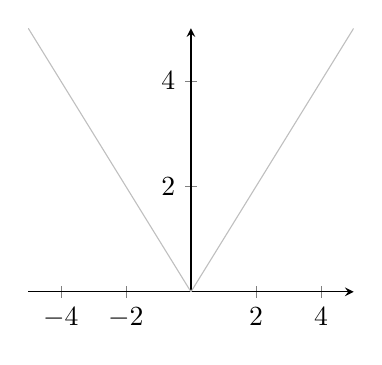
\begin{tikzpicture}
			\begin{axis}[axis lines = center]
				\addplot[color=lightgray]	{abs(x)};
			\end{axis}
		\end{tikzpicture}
	\end{center}
	\caption{The graph $y = |x|$}
\end{figure}


Once again, we present fundamental properties of absolute values, in order to provide a foundation for working with these mathematical functions.

\begin{enumerate}[\hspace{\baselineskip}i.]
	\item For any real number $x$, $|x| \ge x$ and $|x| \ge 0$.
	\item Given real numbers $x$ and $y$, $|xy| = |x| \cdot |y|$.
	\item Squaring a number strips its negative sign, and taking the positive root ensures the result will be positive. Therefore the [positive] square root of the square is the absolute value.
	\begin{align*}
		|x| = \sqrt{x^2}
	\end{align*}
\end{enumerate}

The last property is rather interesting, and can be proved. Notice for proving these simple properties of absolute values, a \emph{proof by cases} \marginnote{proof by cases} is often most effective, a proof technique in which we break all possibilities into distinct \emph{cases} or scenarios and prove the claim for each of them. Since the absolute value function behaves different for positive and negative numbers, these are naturally our cases.

\vspace{\baselineskip}
\begin{theorem}
	For any real number $x$, we have:
	
	\begin{align}
		|x| = \sqrt{x^2}
	\end{align}
\end{theorem}

\begin{proof}[Proof by Cases]
	Consider the cases when $x$ is positive, zero and negative separately. Note formally, one of these cases must be true from the trichotomy property (see the first property of inequalities above).
	
	\header{Case 1.}{$x > 0$}
	
	\begin{align*}
		\sqrt{x^2} &= x \\
		&= |x|
	\end{align*}
	
	\header{Case 2.}{$x = 0$}
	
	\begin{align*}
		\sqrt{0^2} &= 0 \\
		&= |0|
	\end{align*}
	
	\header{Case 3.}{$x < 0$}
	Assume that $x = -a$ for some positive real number $a$. Notice that $|x| = a$ Plugging this into the expression of the square root of the square:
	
	\begin{align*}
		\sqrt{x^2} &= \sqrt{(-a)^2} \\
		&= \sqrt{a^2} \\
		&= a \\
		&= |x|
	\end{align*}
\end{proof}

At this point, we can go ahead and introduce the next major inequality. Note that we mentioned that the absolute value of the product of two numbers is the product of the absolute values, or

\begin{align*}
	|xy| = |x| \cdot |y|.
\end{align*}

Unfortunately, the same does not hold true for sums--the analogous statement is false.

\begin{align*}
	|2 + (-1)| \neq |2| + |-1|
\end{align*}

However, there is a relationship between the two quantities which can be expressed as an inequality. \\

\begin{theorem}[Triangle Inequality]
	Given real numbers $x$, $y$ the sum of the absolute values is always greater than or equal to the absolute value of the sum.
	
	\begin{align}
		|x + y| \le |x| + |y|
	\end{align}
\end{theorem}

\begin{proof}[Rough work]\let\qed\relax
	Once again, we begin with rough work to determine how to progress on the proof. In order to remove the absolute value sides, it seems reasonable to square both sides.
	
	\begin{align*}
		|x + y| &\le |x| + |y| \\
		\implies |x + y|^2 &\le (|x| + |y|)^2 \\
		\implies (x + y)^2 &\le (|x| + |y|)^2 \\
		\implies x^2 + 2xy + y^2 &\le |x|^2 + 2|x||y| + |y|^2 \\
		\implies x^2 + 2xy + y^2 &\le x^2 + 2|xy| + y^2 \\
		\implies xy &\le |xy|
	\end{align*}
	
	Notice we arrived at a statement which is clearly true. Remember that the absolute value of any real number is always greater than or equal to the number. At this point we can write the proof.
\end{proof}

\begin{proof}
	Consider any real number $x$ and $y$. From the basic properties of absolute values we know the product of these numbers must be less than or equal to its absolute value.
	
	\begin{align*}
		xy &\le |xy| \\
		\implies x^2 + 2xy + y^2 &\le x^2 + 2|xy| + y^2 \\
		\implies x^2 + 2xy + y^2 &\le |x|^2 + 2|x||y| + |y|^2 \\
		\implies (x + y)^2 &\le (|x| + |y|)^2 \\
		\implies |x + y|^2 &\le (|x| + |y|)^2
	\end{align*}
	
	Both terms being squared are positive, hence we can safely square root both sides without affecting the inequality.
	
	\begin{align*}
		\therefore |x + y| \le |x| + |y|
	\end{align*}
\end{proof}
\vspace{\baselineskip}

Once again in this proof, we used rough work to arrive at a statement we knew was true, and then worked backward to derive the result we wanted from this true statement. We had to be more careful working backward in this example since we square rooted an inequality. Though this works when both terms inside the square are positive, it may fail spectacularly otherwise.

\begin{align*}
	&4 \ge 1 \\
	\implies (-2)^2 &\ge (1)^2 \\
	\centernot\implies -2 &\ge 1 \text{ false!}
\end{align*}

% ===========================================================
\section{Sets}
% ===========================================================

So far we have been relying on intuition to define the real numbers, the focus of our attention. Although the formal definitions of the real numbers are outside the scope of these notes, it is worth paying attention to this fundamental notion of a group of numbers. In mathematics, this concept is represented as a \emph{set}, \marginnote{set} a well-defined collection of objects. Some examples are listed below.

\begin{align*}
	S = \{\text{Saturday}, \text{Sunday}\} \\
	T = \{1, 2, 3, \dots \} \\
	R = \{n^2 : n \text{ is even} \} \\
	\phi \text{ or } \{ \}
\end{align*}

The last example presents two ways to denote the \emph{empty set}, \marginnote{empty set} the set with no elements. Notice $R$ is the set of squares of all even numbers. The `:' introduces a condition in the set definition. Since every set must be well-defined, every object is either an \emph{element} \marginnote{element} of the set or not. If set $A$ contains element $a$ but does not contain $b$, we can write

\begin{align*}
	a \in A \text{ and } b \notin A.
\end{align*}

In defining sets, we often specify the elements to be included from some \emph{universe} \marginnote{universe} of objects. However, the elements of elements not in $A$ clearly make a set as well, one which is intrinsically linked to $A$. This set is denoted the \emph{complement} \marginnote{complement} of $A$, written as $A^c$ and defined as

\begin{align*}
	A^c = \{ x \in \text{universe } : x \notin A \}
\end{align*}

Though we will explore notions of size in more depth later on, for now we define the \emph{cardinality}, \marginnote{cardinality} written as 

\begin{align*}
	|A| \text{ or } \card(A),
\end{align*}

as its size. For \emph{finite} \marginnote{finite} sets, sets without an infinite number of elements, the cardinality is simply the number of elements. All such cardinalities are in the set $\{0, 1, 2, \dots\}$, with 0 reserved for the empty set.

Since a set is unordered and cannot contain duplicate items, a natural definition of equality is that both sets contain the same elements. On the other hand, if every element of set $B$ is in set $A$, then in some sense the latter set contains the former. Mathematically, we write that $B$ is a \emph{subset} \marginnote{subset} of $A$ or

\begin{align*}
	B \subseteq A.
\end{align*}

Notice under this definition, the empty set is a subset of every set. Similarly, a set is always a subset of itself. In cases where we want to exclude this possibility, that the sets are equal, in explaining the relationship between the two sets, we can write $B$ is a proper subset of $A$ or 

\begin{align*}
	B \subset A
\end{align*}

which means $B \subseteq A$ but $B \neq A$. Along with the real numbers there are a handful of other important sets used to refer to classes of numbers.

\vspace{\baselineskip}
\begin{center}
	\begin{tabular}{ccc}
		\toprule
		Symbol & Name & Set \\
		\midrule
		$\mathbb{N}$ & Natural Numbers & $\{1, 2, 3, 4, \dots\}$ \\[10pt]
		$\mathbb{Z}$ & Integers & $\{\dots, -2, -1, 0, 1, 2, \dots\}$ \\[10pt]
		$\mathbb{Q}$ & Rational Numbers & $\left\{ \dfrac{p}{q} : p,q \in \mathbb{Z}\right\}$ \\[10pt]
		$\mathbb{R}$ & Real Numbers & \\
		\bottomrule
	\end{tabular}
\end{center}
\vspace{\baselineskip}

Notice we defined the natural numbers to exclude 0, but the symbol $\mathbb{N}_0$ could be used to refer to all naturals along with 0. Based on the descriptions of each of these sets, each contains the previous plus some additional elements. Therefore, we can write

\begin{align}
	\mathbb{N} \subseteq \mathbb{N}_0 \subseteq \mathbb{Z} \subseteq \mathbb{Q} \subseteq \mathbb{R}.
\end{align}

Since each set contains the previous, we may wonder what elements are in one but not the other. In some cases, this set itself might be valuable. For example all real numbers which are not rational are  referred to as as \emph{irrational}, \marginnote{irrational} and the set which contains all such numbers the irrational numbers. This set then is a result of taking the real numbers and subtracting away the rational numbers. This operation, along with a few more are formalized before for arbitrary sets $A$ and $B$.

\begin{align*}
	\emph{Subtraction. } A - B &= \{ x \in A : x \notin B \} \\
	\emph{Intersection. } A \cap B &= \{ x : x \in A \text{ and } x \in B \} \\ 
	\emph{Union. } A  \cup B &= \{ x : x \in A \text{ or } x \in B \} \\
	\emph{Cartesian Product. } A  \times B &= \{ (a, b) : a \in A \text{ and } b \in B \} \
\end{align*}

The intersection is the set of all elements in both, while the union is the set of all elements in either. Two sets are called \emph{disjoint} if their intersection is the empty set meaning they have no common elements. Written out this would mean for disjoint sets $S$ and $T$,

\begin{align*}
	S \cap T = \phi
\end{align*}

The cartesian product of two sets outputs a set with a completely different structure: a set of tuples containing all possibly pairs of elements from $A$ and $B$. Unlike sets, \emph{tuples} \marginnote{tuples} are ordered lists of elements which could contain duplicates. This idea of product can be extended beyond two sets.

\begin{align*}
	A \times B &= \{ (a, b) : a \in A, b \in B \} \\
	B \times A &= \{ (b, a) : a \in A, b \in B \} \\
	A \times B \times C &= \{ (a, b, c) : a \in A, b \in B, c \in C \} \\
\end{align*}

Repeated products of the same set can be abbreviated as a power, similar to the real numbers.

\begin{align*}
	A^k &= \underbrace{A \times \cdots \times A}_\text{$k$ times} \\
	&= \{ (a_1, a_2, \dots, a_k) : a_1, a_2, \dots, a_k \in A \}
\end{align*} 

One final concept that must be introduced to complete our discussion on introductory set theory is the \emph{power set} \marginnote{power set} of a set, which contains all possible subsets. Formally we write this as

\begin{align*}
	\emph{Power set. } \mathcal{P}(A) = \{ S : S \subseteq A \}.
\end{align*}

To ensure this section includes a proof, we end with a simple theorem about the size of a power set. We will explore another proof of this theorem later in the course.

\vspace{\baselineskip}
\begin{theorem}
	For a finite set $A$, if $|A| = n$, then its power set $\mathcal{P}(A)$ has cardinality $2^n$.
\end{theorem}

\begin{proof}[Examples]\let\qed\relax
	One way to begin working on a proof is the test the claim with examples, since they may yield insight into why the result is true.
	
	\begin{align*}
		\mathcal{\phi} &= \{ \phi \} \\
		\mathcal{P}(\{ 0, 1 \}) &= \{ \phi, \{ 0 \}, \{ 1 \}, \{ 0, 1 \}\}
	\end{align*}
	
	In each of these cases, the result holds. When the sizes of sets were 0 and 2, their power sets had sizes of 1 and 4 respectively. Notice we would also expect the number of subsets to be even, since for every subset $S \subseteq A$, $(A - S)$ is also one, and  this theorem seems to check out in that regard. At this point we can present the proof
\end{proof}

\begin{proof}
	Since $A$ is finite and $|A| = n$ then the set must have $n$ elements. Let us arbitrarily assign labels so that
	
	\begin{align*}
		A = \{ a_1, a_2, \dots a_n \}
	\end{align*}
	
	In constructing a subset, each of these $n$ distinct elements can be chosen to either be included or excluded from the set. Since every subset can be created with these series of $n$ choices, and each choice has two options, the number of subsets is $2^n$.
\end{proof}
\vspace{\baselineskip}

A major class of proofs involves proving two sets are equal. One possible way of doing this involves showing each set is a subset of another. To prove set $S$ is a subset of $T$, we must show if $x$ is an element of $S$ then it is also an element of $T$. This would mean every element in $S$ is contained in $T$ and therefore $S \subseteq T$. To provide an example, we introduce another theorem. \\

\begin{theorem}[De Morgan's laws]
	Given two sets $A$ and $B$, the following statements are true.
	
	\begin{align}
		(A \cup B)^c &= A^c \cap B^c \\
		(A \cap B)^c &= A^c \cup B^c
	\end{align}
\end{theorem}

\begin{proof}
	Since the proof the statements are nearly identical, only the first will be proved; the second is left as an exercise. Since we are proving the equality of sets, we proceed by showing the left-hand side (LHS) is a subset of the right-hand side (RHS) and vice versa.
	
	\header{Part 1.}{$(A \cup B)^c \subseteq (A^c \cap B^c)$}
	
	Assume that $x \in (A \cup B)^c$, we will show $x$ is also an element of $(A^c \cap B^c)$ through a series of implications.
	
	\begin{align*}
		x \in (A \cup B)^c &\implies x \notin (A \cup B) \\
		&\implies x \notin A \text{ and } x \notin B \\
		&\implies x \in A^c \text{ and } x \in B^c \\
		&\implies x \in A^c \cap B^c
	\end{align*}
		
	\header{Part 2.}{$(A^c \cap B^c) \subseteq (A \cup B)^c$}
	
	Now assume that $x \in (A^c \cap B^c)$, we will show $x$ is also an element of $x \in (A \cup B)^c$.
	
	\begin{align*}
		x \in (A^c \cap B^c) &\implies x \in A^c \text{ and } x \in B^c \\
		&\implies x \notin A \text{ and } x \notin B \\
		&\implies x \notin (A \cup B) \\
		&\implies x \in (A \cup B)^c
	\end{align*}
	
	Since we have proved that $(A \cup B)^c \subseteq (A^c \cap B^c)$ and $(A^c \cap B^c) \subseteq (A \cup B)^c$, this is enough to show equality.
	
	\begin{align*}
		\therefore (A \cup B)^c &= A^c \cap B^c
	\end{align*}
\end{proof}
\vspace{\baselineskip}

% ===========================================================
\section{Functions}
% ===========================================================

At this point we can introduce a very special type of set which has profound uses in mathematics. This, of course, is a \emph{function}, \marginnote{function} which is a set of input-output ordered pairs which can represented as

\begin{align*}
	\{ (x, f(x)) : x \in \text{domain} \}	
\end{align*}

\begin{center}
	\begin{tabular}{rl}
		\toprule
		Term & Definition \\
		\midrule
		Domain & The set of all allowed inputs \\
		Codomain (Target Space) & The set of all allowed outputs \\
		Image (Range) & The set of all actual outputs \\
		\bottomrule
	\end{tabular}
\end{center}
\vspace{\baselineskip}

The function, then, takes an input from the domain and returns a single output in the codomain. This property of linking the domain to the codomain explains why function are often called \emph{maps}. \marginnote{map} Since the image is the set of outputs, and a subset of the codomain, it would be the set that results from applying the function to every element in the domain. Thus, for a function $f$ with domain $A$, the image is often denoted as $f(A)$.

\begin{align*}
	f(A) &= \{ f(a) : a \in A \}
\end{align*}

In defining a function, the domain and codomain must be explicitly specified, hence the following notation is often used.

\begin{align*}
	\begin{array}{llll}
		\multicolumn{4}{l}{\text{domain}} \\
		& \downarrow && \\
		f: & A & \rightarrow & B \\
		&&& \uparrow \\
		\multicolumn{4}{r}{\text{codomain}}
	\end{array}
\end{align*}

A function is called \emph{real-valued} \marginnote{real-valued} if its image is a subset of the real numbers, and thus all its outputs are real numbers. The \emph{graph} \marginnote{graph} of a function is a plot of all the input-output pairs. In working with functions there are a few elementary ways to combine them.

\begin{align}
	\emph{Addition. } (f + g)(x) = f(x) + g(x) \\
	\emph{Multiplication. } (f \cdot g)(x) = f(x) \cdot g(x) \\
	\emph{Composition. } (f \circ g)(x) = f(g(x))
\end{align}

We are often extremely interested in the image of a real-valued function. In particular, we may wonder about the nature of this set: does it have a maximum or minimum, or does the function go to infinity? Formally, a function $f: A \rightarrow \mathbb{R}$ is \emph{bounded} \marginnote{bounded} if there exists some $M \in \mathbb{R}$ such that

\begin{align*}
	|f(x)| \le M
\end{align*}

for all $x \in A$. Notice in this definition $M$ acts both a positive and negative bound since the statement is equivalent to

\begin{align*}
	-M \le f(x) \le M.
\end{align*}

It turns out that sums and products of bounded functions are bounded as well, results we prove below. Notice in these proofs we clearly state our assumptions and what we plan on showing, a technique that helps inform our approach.

\vspace{\baselineskip}
\begin{theorem}
	If functions $f$ and $g$ are bounded so are the functions $(f \cdot g)$ and $(f + g)$, formed by the sum and product of these functions respectively.
\end{theorem}

\begin{proof}
	Since $f$ and $g$ are bounded, there exist $M \in \mathbb{R}$ and $N \in \mathbb{R}$ for which 
	
	\begin{align*}
		|f(x)| \le M \text{ and } |g(x)| \le N.
	\end{align*}
	
	We hope to show there exists some bound on $|(f \cdot g)(x)|$, therefore our aim should be to express this in terms of the quantities we already have bounds for.
	
	\begin{align*}
		|(f \cdot g)(x)| &= |f(x) \cdot g(x)| \\
		&= |f(x)| \cdot |g(x)| \\
		&\le M \cdot N
	\end{align*}
	
	This shows that we have discovered a bound for the function: the product of the two bounds of our original function. Hence the function is bounded.
\end{proof}

\begin{proof}
	Once again, assume there exist $M \in \mathbb{R}$ and $N \in \mathbb{R}$ for which
	
	\begin{align*}
		|f(x)| \le M \text{ and } |g(x)| \le N.
	\end{align*}
	
	We wish to find a bound for $|(f + g)(x)|$. However, in this case it is more tricky to decompose this into $|f(x)|$ and $|g(x)|$, and requires the triangle inequality.
	
	\begin{align*}
		|(f + g)(x)| &= |f(x) + g(x)| \\
		&\le |f(x)| + |g(x)| \\
		&\le M + N
	\end{align*}
	
	Thus, we have proved $(f + g)$, showing the sum of the bounds of the functions is the bound for the sum of the functions.
\end{proof}
\vspace{\baselineskip}

In general, approach bounding proofs by expressing the bounded functions by their definitional inequality. Then work on manipulating these inequalities through inequality or absolute value rules to obtain the desired result.

% ===========================================================
\section{Fields}
% ===========================================================

So far in our deals with $\mathbb{R}$, we have been implicitly relying on properties or axioms of arithmetic in the real numbers. Many of these properties are not exclusive to the reals, and apply to a class of algebraic structures called \emph{fields}. \marginnote{field} A field, $F$, consists of

\begin{align*}
	(F, 0, 1, +, \cdot) \text{ where } F = \{ 0, 1, \dots \}. 
\end{align*}

$F$ is a set of elements in the field in including at least the additive identity 0 and the multiplicative identity 1. A field also includes two predefined binary operations, addition and multiplication, which take two inputs in $F$ and return the sum and product in $F$ respectively. These function must obey the following axioms for $x, y, z \in F$.

\begin{align*}
	+: F \times F \rightarrow F \\
	\cdot: F \times F \rightarrow F
\end{align*}

\begin{center}
	\begin{tabular}{rp{1.5in}p{1.5in}}
		\toprule
		Name & Addition & Multiplication \\
		\midrule
		\emph{Closure} & $x + y \in F$ & $x \cdot y \in F$ \\
		\emph{Associativity} & $(x + y) + z = x + (y + z)$ & $(x \cdot y) \cdot z = x \cdot (y \cdot z)$ \\
		\emph{Commutativity} & $x + y = y + x$ & $x \cdot y = y \cdot x$ \\
		\emph{Identity} & $x + 0 = x$ & $x \cdot 1 = x$ \\
		\emph{Inverses} & each non-zero element has an additive inverse & each element has an multiplicative inverse \\[10pt]
		\emph{Distributivity} & \multicolumn{2}{c}{$x \cdot (y + z) = x 
\cdot y + x \cdot z$} \\
		\bottomrule
	\end{tabular}
\end{center}
\vspace{\baselineskip}

To clarify the inverse axioms, the first states that for any $x \in F$, there exists a $-x$ in the field, such that

\begin{align*}
	x + (-x) = 0, \, -x \in F.
\end{align*}

In this case, $-x$ is simply an element of the field, and is called the additive inverse of $x$. Commutatively, $x$ is the additive inverse of $-x$. Sometimes, the additive inverse of a field element is itself--the trivial example is 0:

\begin{align*}
	0 + 0 = 0.
\end{align*}

For non-zero elements in the field, a multiplicative inverse exists as well, which means for $x \in F - \{ 0 \}$, there exists a $x^{-1}$, such that

\begin{align*}
	x \cdot x^{-1} = 1,\, x^{-1} \in F.
\end{align*}

Similar to the additive inverse, this inverse is an element of the field and likewise can be the same number. With this axiom, we can define two new operations in the field. Subtraction amounts to adding by the additive inverse and division is multiplication by the multiplicative inverse. For field elements $x$, $y$ in some field $F$.

\begin{align}
	x - y &:= x + (-y) \\
	x / y &:= x \cdot y^{-1} \text{ given } y \neq 0
\end{align}

Notice the $:=$ here emphasizes the expression on the left is defined to be equal to the expression on the right. To avoid confusion, when working in fields, we will refrain from using subtraction and division and instead refer to the inverses.

Naturally, we may now wonder, having laid out these axioms, which sets which classes of numbers, with regularly defined addition and multiplication, constitute fields. To prove whether a set with defined operations is a field is simply a matter of checking each of the axioms. \\

\vspace{\baselineskip}
\begin{theorem}
	The natural numbers $(\mathbb{N})$ and integers $(\mathbb{Z})$ are not fields. 
\end{theorem}

\begin{proof} 
	We will prove this theorem in two parts, first dealing with the natural numbers proceeded by the integers.
	\header{Part 1. }{$\mathbb{N}$}
	The additive inverse axiom fails for all integers. Specifically, the number 1, for example, has no additive inverse since for all $n \in \mathbb{N}, 1 + n > 0$. Since 1 had no additive inverse this is not a field.
	
	\header{Part 2. }{$\mathbb{Z}$}
	The multiplicative inverse axiom fails for $2 \in \mathbb{Z}$. Once way of rigourously showing this is to notice $2 \cdot n$ is even for all $n \in \mathbb{Z}$. Therefore this value can never be 1, and hence no multiplicative inverse exists. \\
\end{proof}
\vspace{\baselineskip}

\vspace{\baselineskip}
\begin{theorem}
	The rational numbers $(\mathbb{Q})$ and real numbers $(\mathbb{R})$ with regularly defined addition and multiplication constitute fields.
\end{theorem}

\begin{proof}
	The process of proving these are fields are rather tedious, verifying each of the field axioms individually, and left as an exercise. However, note that the inverse axioms that failed for the natural numbers and integers hold for these two sets. The additive and multiplicative inverses are respectively shown below.
	
	\begin{align*}
		\frac{p}{q} \in \mathbb{Q} \rightarrow -\frac{p}{q}, \, \frac{q}{p} \in \mathbb{Q} \\
		x \in \mathbb{R} \rightarrow -x, \, \frac{1}{x} \in \mathbb{R}
	\end{align*}
\end{proof}
\vspace{\baselineskip}

These suite of axioms lead to a host of simple properties, which should feel familiar to us after working with the real numbers. We introduce an expansive theorem which lays out many of these properties.

\vspace{\baselineskip}
\begin{theorem}
	Given a field $F$ defined with addition and multiplication and three elements $x$, $y$, and $z$, the following properties must hold.
	
	\begin{align}
		x \cdot 0 = 0 \\
		\text{if } x \cdot y = 0 \text{ then } x = 0 \text { or } y = 0 \\
		-x = x \cdot (-1) \\
		(-x) \cdot (-y) = x \cdot y \\
		\text{if } x + y = x + z \text{ then } y = z \\
		\text{if } x \cdot y = x \cdot z \text{ then } y = z \text { if } x \neq 0
	\end{align}
\end{theorem}

\begin{proof}
	Proving every statement in the theorem would take up a lot of space, hence we will present proofs for the first and last statement, hopefully providing a model for approaching proofs to the remaining statements.
	
	\header{Statement 1.18. }{$x \cdot 0 = 0$}
	
	Notice that although we take this for grated in the real numbers, it is not a field axiom and must be proved. Since 0 is the additive inverse, in searching for a proof we should look to exploit its properties.

	\begin{align*}
		x \cdot 0 &= x \cdot (0 + 0) &&\emph{identity} \\
		&= x \cdot 0 + x \cdot 0 &&\emph{distributive}
	\end{align*}
	
	At this point notice by closure we know $x \cdot 0$ lies within the field. Therefore, by the inverses axiom it must have an additive inverse. Now we add this to both sides of the equation.
	
	\begin{align*}
		x \cdot 0 + x \cdot 0 &= x \cdot 0 && \\
		x \cdot 0 + x \cdot 0 + (-(x \cdot 0)) &= x \cdot 0 + (-(x \cdot 0)) && \\
		x \cdot 0 + (x \cdot 0 + (-(x \cdot 0))) &= 0  &&\emph{associative} \\
		x \cdot 0 + 0 &= 0 &&\emph{inverse} \\
		x \cdot 0 &= 0 &&\emph{identity}
	\end{align*}
	
	This is the result we were looking for. Notice instead of subtracting $x \cdot 0$ from each side, as we would in the real numbers, we added the additive inverse to  both sides. In this proof we clearly listed which axiom allowed us to make each step, and although this is not necessary, it makes it less likely to perform an operation which is not allowed.
	
	\header{Statement 1.23. }{$\text{if } x \cdot y = x \cdot z \text{ then } y = z \text { if } x \neq 0$}
	
	Once again, we attempt a direct proof based on the field axioms. Since $x \neq 0$ from the inverses axiom, we know there exists some $x^{-1} \in F$ such that
	
	\begin{align*}
		x \cdot x^{-1} = 1
	\end{align*}
	
	We simply multiply both sides of out equation with this term.
	
	\begin{align*}
		x \cdot y &= x \cdot z && \\
		x^{-1} \cdot x \cdot y &= x^{-1} \cdot x \cdot z && \\
		(x^{-1} \cdot x) \cdot y &= (x^{-1} \cdot x) \cdot z &&\emph{associativity} \\
		1 \cdot y &= 1 \cdot z &&\emph{inverse} \\
		y &= z &&\emph{identity}
	\end{align*}
	
	Once again, we have arrived at our result, hence we have proved this this statement for arbitrary fields. Notice we could approach this problem as if we were asked to prove this for real numbers. Instead of dividing both sides by $x$ we multiplied by $x^{-1}$ to arrive at the result. 
\end{proof}
\vspace{\baselineskip}

The two fields we have discussed so far have had an infinite number elements with predefined addition and multiplication operations that mirror their common usage. However, we may wonder what other fields exists, and in particular, what such a field would look like for a finite number of elements, a \emph{finite field}. \marginnote{finite field} Since a field must have at least two elements, let us attempt to construct a two element field, called the \emph{binary field}. \marginnote{binary field} Consider the field

\begin{align*}
	(S, 0, 1, +, \cdot) \text{ where } S = \{ 0, 1 \}.
\end{align*}
	
Unfortunately, we must define multiplication and addition in this field since otherwise the latter would defy the closure field axiom as

\begin{align*}
	1 + 1 &= 2 \notin S.
\end{align*}

For finite fields with a small number of elements, the most effective method of defining these operations involves writing addition and multiplication tables, providing outputs for all possible pairs of input for each function.

\vspace{\baselineskip}
\begin{center}
\begin{TAB}(e, 15pt){c|cc}{c|cc}
	+ & 0 & 1 \\
	0 & & \\
	1 & &
\end{TAB}
\hspace{15pt}
\begin{TAB}(e, 15pt){c|cc}{c|cc}
	$\cdot$ & 0 & 1\\
	0 & & \\
	1 & & \\
\end{TAB}
\end{center}
\vspace{\baselineskip}

Notice, that multiplying by 0 always returns 0 (as we proved above) and multiplying by 1 gives the same number. Similarly, adding 0 returns the same number by the identity property. 

\vspace{\baselineskip}
\begin{center}
\begin{TAB}(e, 15pt){c|cc}{c|cc}
	+ & 0 & 1 \\
	0 & 0 & 1 \\
	1 & 1 &
\end{TAB}
\hspace{15pt}
\begin{TAB}(e, 15pt){c|cc}{c|cc}
	$\cdot$ & 0 & 1\\
	0 & 0 & 0 \\
	1 & 0 & 1 \\
\end{TAB}
\end{center}
\vspace{\baselineskip}

This only leaves one output to be decided, the sum $1 + 1$. In the next theorem we prove that this is equal to 0. To do this, we introduce a new type of proof, a proof by contradiction.

\vspace{\baselineskip}
\begin{theorem}
	If $S$ is the binary field with $S = \{ 0, 1\}$, then $1 + 1 = 0$.
\end{theorem}

\begin{proof}[Proof by Contradiction]
	By the closure property of fields, we know the sum $1 + 1$ must lie within $S$ and is therefore it is either 0 or 1. Assume for sake of contradiction that it is indeed 1, so that
	
	\begin{align*}
		1 + 1 = 1.
	\end{align*}
	
	By the inverse axiom, we know that 1 has an additive inverse in the field. We now add this inverse to both sides of the equation.
	
	\begin{align*}
		1 + 1 + (-1) &= 1 + (-1) \\
		1 + 0 &= 0 \\
		1 &= 0
	\end{align*}
	
	This is clearly false since by definition a field must have distinct elements 0 and 1. Since this would be a logical consequence of letting $1 + 1 = 1$, that assumption must be false. Hence we are left only with the possibility that
	
	\begin{align*}
		1 + 1 = 0.
	\end{align*}
\end{proof}
\vspace{\baselineskip}

In a \emph{proof by contradiction}, we assume the opposite of the statement we are trying to prove, and show how this leads a result that is clearly false. This \emph{contradiction} \marginnote{contradiction} shows that our initial assumption must be false, and therefore its opposite true. In this way, we indirectly prove our claim is true by showing it cannot be false. In the last proof, we demonstrated if $1 + 1 = 1$ then $0 = 1$, which is clearly false. Therefore, we could conclude $1 + 1 \neq 1$, which meant $1 + 1 = 0$, what we wanted to show.

Moving on, we can tackle the construction of three-element field $T = \{ 0, 1, \omega \}$. Immediately, we write the addition and multiplication tables and fill out the simple rows and columns.

\vspace{\baselineskip}
\begin{center}
\begin{TAB}(e, 15pt){c|ccc}{c|ccc}
	+ & 0 & 1 & $\omega$\\
	0 & 0 & 1 & $\omega$ \\
	1 & 1 & & \\
	$\omega$ & $\omega$ &&
\end{TAB}
\hspace{15pt}
\begin{TAB}(e, 15pt){c|ccc}{c|ccc}
	$\cdot$ & 0 & 1 & $\omega$\\
	0 & 0 & 0 & 0 \\
	1 & 0 & 1 & $\omega$ \\
	$\omega$ & 0 & $\omega$ &
\end{TAB}
\end{center}
\vspace{\baselineskip}

Completing the multiplication table is simple; since every element in the field must have a multiplicative inverse, in the case of $\omega$, this must be itself. In other words, every non-zero row or column in a field multiplication table must have a single 1.

\vspace{\baselineskip}
\begin{center}
\begin{TAB}(e, 15pt){c|ccc}{c|ccc}
	+ & 0 & 1 & $\omega$\\
	0 & 0 & 1 & $\omega$ \\
	1 & 1 & & \\
	$\omega$ & $\omega$ &&
\end{TAB}
\hspace{15pt}
\begin{TAB}(e, 15pt){c|ccc}{c|ccc}
	$\cdot$ & 0 & 1 & $\omega$\\
	0 & 0 & 0 & 0 \\
	1 & 0 & 1 & $\omega$ \\
	$\omega$ & 0 & $\omega$ & 1
\end{TAB}
\end{center}
\vspace{\baselineskip}
	
This leaves the addition table to be completed, to do this we introduce a new theorem which helps complete the non-diagonal entries.

\vspace{\baselineskip}
\begin{theorem}
	For a three-element field $(T, 0, 1, +, \cdot)$ with $T = \{ 0, 1, \omega \}$ the following equation must be true.
	
	\begin{align*}
		1 + \omega &= 0 \\
	\end{align*}
\end{theorem}

\begin{proof}[Proof by Contradiction]
	Assume for sake of contradiction that $1 + \omega \neq 0$. Then, by closure the sum must either be $\omega$ or 1. We would show either case results in a contradiction.
	
	\header{Case 1.}{$1 + \omega = 1$}
	
	Since 1 is in the field, the inverses property tells us that an additive inverse exists. Adding both sides with this additive inverse we immediately see the contradiction.
	
	\begin{align*}
		1 + \omega &= 1 \\
		(-1) + 1 + \omega &= 1 + (-1) \\
		\omega &= 0
	\end{align*}
	
	Since the elements are distinct this is a contradiction.

	\header{Case 2.}{$1 + \omega = \omega$}
	
	We approach this case in a very similar way, clearing the $\omega$'s from both sides to expose a contradiction.
	
	\begin{align*}
		1 + \omega &= \omega \\
		1 + \omega + (-\omega) &= \omega + (-\omega) \\
		1 &= 0
	\end{align*}
	
	This again, is a contradiction. Therefore in the absence of any alternatives, we have proved that $1 + \omega = 0$
\end{proof}
\vspace{\baselineskip}

Note in this proof, we applied a case-by-case approach to a proof by contradiction. This is analogous to a proof by cases where we prove the result in every case, except we actually show a contradiction in each case.

\vspace{\baselineskip}
\begin{center}
\begin{TAB}(e, 15pt){c|ccc}{c|ccc}
	+ & 0 & 1 & $\omega$\\
	0 & 0 & 1 & $\omega$ \\
	1 & 1 & & 0 \\
	$\omega$ & $\omega$ & 0 &
\end{TAB}
\hspace{15pt}
\begin{TAB}(e, 15pt){c|ccc}{c|ccc}
	$\cdot$ & 0 & 1 & $\omega$\\
	0 & 0 & 0 & 0 \\
	1 & 0 & 1 & $\omega$ \\
	$\omega$ & 0 & $\omega$ & 1
\end{TAB}
\end{center}
\vspace{\baselineskip}
	
The remaining two spaces are rather easy to fill out if we remember the property that in a field

\begin{align*}
	\text{if } x + y = x + z \text{ then } y = z
\end{align*}

Fixing $x$ by focusing on an individual role or column, this tells us that different entries must be different. This is because, for example,

\begin{align*}
	\text{if } 1 + 1 = 1 + \omega \text{ then } 1 = \omega.
\end{align*}

Interestingly, this means every row and column of the addition table must contain each of the field elements. Exploiting the analogous rule for multiplication, every non-zero row or column must have every field element appear exactly once. Armed with this knowledge, we can finally complete the operator definitions, showing a three-element field exists.

\begin{align*}
	T = \{ 0, 1, \omega \}
\end{align*}

\begin{center}
\begin{TAB}(e, 15pt){c|ccc}{c|ccc}
	+ & 0 & 1 & $\omega$\\
	0 & 0 & 1 & $\omega$ \\
	1 & 1 & $\omega$ & 0 \\
	$\omega$ & $\omega$ & 0 & 1
\end{TAB}
\hspace{15pt}
\begin{TAB}(e, 15pt){c|ccc}{c|ccc}
	$\cdot$ & 0 & 1 & $\omega$\\
	0 & 0 & 0 & 0 \\
	1 & 0 & 1 & $\omega$ \\
	$\omega$ & 0 & $\omega$ & 1
\end{TAB}
\end{center}
\vspace{\baselineskip}

% ===========================================================
\section{Exercises}
% ===========================================================

\begin{enumerate}[(a)]
	\setlength\itemsep{\baselineskip}
	\item  Prove that for two real numbers $x$ and $y$, $|x - y| \ge |x| - |y|$.
	
	\item Given $x + 2y = 100$, determine the maximum value of $xy$ using the arithmetic-geometric mean inequality.
	
	\item For real numbers $x, y, u, v,$ show that 
	\begin{align*}
		(xu + yv)^2 \le (x^2 + y^2)(u^2 + v^2).
	\end{align*}

	\item When does equality hold for the triangle inequality? In other words, for what values of $x$ and $y$ does 
	\begin{align*}
		|x + y| = |x| + |y|?
	\end{align*}

	\item Prove for any $a, b > 0$ the following inequality holds true.
	\begin{align*}
		\frac{4}{ab} \le \left( \frac{1}{a} + \frac{1}{b} \right)^2	
	\end{align*}

	\item Prove the following for three real numbers $x$, $y$, and $z$.
	\begin{align*}
		|x + y + z| \le |x| + |y| + |z|
	\end{align*}
	
	\item Show the image of the function $f$ is the set (0, 1], for
	\begin{align*}
		f: \mathbb{R} \rightarrow \mathbb{R}, \, f(x) = \frac{1}{x^2 + 1}.
	\end{align*}
	
	\item Let $C$ and $D$ be sets in the domain of $g$. Prove the following relationship about the images of the function.
	\begin{align*}
		g(C \cap D) \subseteq g(C) \cap g(D)
	\end{align*}
	
	\item Let $f$ and $g$ be two bounded functions. Which of the following functions are also bounded?
	\begin{align*}
		f + g, \, f \cdot g, \, \frac{f}{g}, \, \frac{1}{f^2 + 1}
	\end{align*}
	
	\item If $(f - g)$ and $(f \cdot g)$ are bounded, prove that the function $(f + g)$ is bounded.
	
	\item Consider the four element field $F = \{0, 1, a, b\}$ with operations $+$ and $\cdot$. Complete the addition and multiplication tables below, if possible, and determine the number of different fields which satisfy the axioms.
	
	\vspace{\baselineskip}
	\begin{center}
		\begin{TAB}(e, 15pt){c|cccc}{c|cccc}
			+ & 0 & 1 & $a$ & $b$ \\
			0 & & & & \\
			1 & & & & \\
			$a$ & & & & \\
			$b$ & & & &
		\end{TAB}
		\hspace{15pt}
		\begin{TAB}(e, 15pt){c|cccc}{c|cccc}
			$\cdot$ & 0 & 1 & $a$ & $b$ \\
			0 & & & & \\
			1 & & & & \\
			$a$ & & & & \\
			$b$ & & & &
		\end{TAB}
	\end{center}
	\vspace{\baselineskip}
	
	\item For each of the statements below either provide a proof or counterexample. (1) For any $x \in S$, we have $x \cdot 0 = 0$, and (2) $y \cdot 1^{-1} = y^{-1}$ for any $y \neq 0$ in $S$.
\end{enumerate}

\chapter{Language and Proofs}

% ===========================================================
\section{Statements and Connectives}
% ===========================================================

The atomic unit of mathematical reasoning is the \emph{mathematical statement} or \emph{proposition}, \marginnote{proposition} a sentence that is either true or false. This requirement is called the \emph{principle of bivalence.} For a statement, its \emph{truth value} is whether it is true or false. Examples of statements are given below.

\begin{align*}
	P &\equiv \text{$\pi$ is rational} \\
	Q &\equiv \text{$x^2 + x + 1$ has a real solution} \\
	R &\equiv \text{July 4, 1776 was a Thursday} \\
\end{align*}
 
In our examples, the first statement is false while the other two are true. On the other hand ``let them eat cake'' is not a mathematical statement. These statements can be combined with logical connectives to express more complicated thoughts, which are listed below.

\vspace{\baselineskip}
\begin{center}
	\begin{tabular}{ccc}
		\toprule
		Name & Usage & Meaning \\
		\midrule
		Negation & $\neg P$ & not $P$ \\
		Conjunction & $P \wedge Q$ & $P$ and $Q$ \\
		Disjunction & $P \lor Q$ & $P$ or $Q$ \\
		Conditional & $P \implies Q$ & if $P$ then $Q$ \\
		Biconditional & $P \iff Q$ & $P$ if and only if $Q$ \\
		\bottomrule
	\end{tabular}
\end{center} 
\vspace{\baselineskip}

Similar to defining operators in a finite field, we provide rigorous definitions for these logical connectives by showing whether the compound statement is true of false for every possible set input. Fortunately there are very few possible inputs since each statement can either be true or false. In composing a table, called a \emph{truth table}, \marginnote{truth table} we let each row correspond to a unique input.

\vspace{\baselineskip}
\begin{center}
	\begin{TAB}(c, 50pt){cc}{c|cc}
		$P$ & $\neg P$ \\
		T & F \\
		F & T \\
	\end{TAB}
\end{center}
\vspace{\baselineskip}

Notice this truth table shows completely negation, since it tells us how the statement behaves given every input. In this case, if a statement is true its negation is false and if a statement is false its negation is true. In English, then, the negation of a statement would be its opposite. The truth tables for the remaining connective are given below; notice each require two inputs and thus have four possible inputs.

\vspace{\baselineskip}
\begin{multicols}{2}
	\begin{center}
	\begin{TAB}(c, 50pt){ccc}{c|cccc}
		$P$ & $Q$ & $P \wedge Q$ \\
		T & T & T \\
		T & F & F \\
		F & T & F \\
		F & F & F \\
	\end{TAB}
	\end{center}
	
	\begin{center}
	\begin{TAB}(c, 50pt){ccc}{c|cccc}
		$P$ & $Q$ & $P \implies Q$ \\
		T & T & T \\
		T & F & F \\
		F & T & T \\
		F & F & T \\
	\end{TAB}
	\end{center}
	
	\begin{center}
	\begin{TAB}(c, 50pt){ccc}{c|cccc}
		$P$ & $Q$ & $P \lor Q$ \\
		T & T & T \\
		T & F & T \\
		F & T & T \\
		F & F & F \\
	\end{TAB}
	\end{center}

	\begin{center}
	\begin{TAB}(c, 50pt){ccc}{c|cccc}
		$P$ & $Q$ & $P \iff Q$ \\
		T & T & T \\
		T & F & F \\
		F & T & F \\
		F & F & T \\
	\end{TAB}
	\end{center}
\end{multicols}
\vspace{\baselineskip}

These truth tables provide complete definitions for each of these operators, but fail to provide very much intuition.

\begin{enumerate}[\hspace{\baselineskip}i.]
	\item \emph{Negation:} As mentioned before, if $R$ is true its negation is false and vice versa. The simple interpretation of this that $\neg R$ is the opposite of $R$.
	\begin{align*}
		P &\equiv \text{$\pi$ is rational} \\
		\neg P &\equiv \text{$\pi$ is not rational} \\
		Q &\equiv \sqrt{2} > 0 \\
		\neg Q &\equiv \sqrt{2} \le 0
	\end{align*}
	
	\item \emph{Conjunction:} $P \wedge Q$ is true only when both $P$ and $Q$ are true, which matches with we think about ``and.''
	\begin{align*}
		P &\equiv \text{$\sqrt{2}$ is irrational} \\
		Q &\equiv \text{$(x^2 = 2)$ holds when $x = \sqrt{2}$} \\
		P \wedge Q &\equiv \text{$\sqrt{2}$ is irrational and a solution to $x^2 = 2$}
	\end{align*}

	\item \emph{Disjunction:} $P \lor Q$ is true when either $P$, $Q$, or both $P$ and $Q$ are true. Another way to think about this is that  $P \lor Q$ is only false when both statements $P$ and $Q$ are both false. There is a slight difference between this logical ``or'' and the one in everyday usage; often times, ``or'' in English can mean one or the other but not both, which would be called the \emph{exclusive-or} in mathematics.
	\begin{align*}
		P &\equiv \text{$x$ is positive} \\
		Q &\equiv \text{$x$ is negative} \\
		P \lor Q &\equiv \text{$x$ is positive or negative} \\
		&\equiv \text{$x$ is nonzero}
	\end{align*}
	
	\item \emph{Conditional:} This connective is essential in proofs, and thus is worth taking closer look at.
	\begin{align*}
	\begin{array}{lll}
		\multicolumn{3}{l}{\text{hypothesis}} \\
		\downarrow && \\
		P & \implies & Q \\
		&& \uparrow \\
		\multicolumn{3}{r}{\text{conclusion}}
	\end{array}
	\end{align*}
	The first statement is called the \emph{hypothesis}\marginnote{hypothesis} and the second statement the \emph{conclusion}\marginnote{conclusion}. The statement $(P \implies Q)$, interpreted as either
	
	\vspace{\baselineskip}
	\begin{center}
			``if $P$ then $Q$'' or \\
			``$P$ implies $Q$,''
	\end{center}
	\vspace{\baselineskip}
	
	  means when $P$ (the hypothesis) is true, $Q$ (the conclusion) must be true as well. On the other hand, when $P$ is false, it does matter whether $Q$ is true or false, and the statement is true in either case. Once again, the only time a conditional is false is when $P$ is true but $Q$ is false.
	  
	  \item \emph{Biconditional:} A biconditional $(P \iff Q)$ is true when both $P$ and $Q$ have the truth value and false they do not. Therefore, if the biconditional is true the statements $P$ and $Q$ are logically interchangeable since both are true or false together. For this reason, $P$ and $Q$ can be said to be ``logically equivalent.'' This concept can be expressed in two ways as either
	  	  
	  \begin{align*}
	  	P \iff Q \text{ or } P \equiv Q,
	  \end{align*}
	  
	  where the second notation is traditionally used to indicate the two logical compound expressions are equivalent, especially when one side might itself contain the biconditional connective.
\end{enumerate}

It turns out that from these logical connective we can construct many expressions which are identical. We prove a few of the important logical equivalences. \\

\begin{theorem}[De Morgan's laws]
	For two logical statements $R$ and $S$, the following equivalences are true.
	
	\begin{align}
		\neg(R \wedge S) &\equiv \neg R \lor \neg S \\
		\neg(R \lor S) &\equiv \neg R \wedge \neg S
	\end{align}
\end{theorem}

\begin{proof}
	The general way to prove logical statements are equivalent is to construct truth tables and show both statements have identical outputs for the same inputs. In order to avoid receptiveness, we will do this for the first statement and leave the proof of the second as an exercise.
	
	\vspace{\baselineskip}
	\begin{center}
		\begin{tabular}{cccc}
			$R$ & $S$ & $R \wedge S$ & $\neg(R \wedge S)$ \\
			\midrule
			T & T & T & F \\
			T & F & F & T \\
			F & T & F & T \\
			F & F & F & T \\
		\end{tabular}
	\end{center}
	\vspace{\baselineskip}
	
	This gives us the truth table for the left-hand side of the equation. We follow the same process, slow building up the right-hand side.
	
	\vspace{\baselineskip}
	\begin{center}
		\begin{tabular}{ccccc}
			$R$ & $S$ & $\neg R$ & $\neg S$ & $\neg R \lor \neg S$ \\
			\midrule
			T & T & F & F & F \\
			T & F & F & T & T \\
			F & T & T & F & T \\
			F & F & T & T & T \\
		\end{tabular}
	\end{center}
	
	Since $(\neg R \lor \neg S)$ and $\neg(R \wedge S)$ are true and false together, given the same inputs (have identical columns) the two statements are logically equivalent. \\
\end{proof}
\vspace{\baselineskip}

\vspace{\baselineskip}
\begin{theorem}
	The following important logical equivalences are also true.
	
	\begin{align}
		P \iff Q &\equiv (P \implies Q) \wedge (Q \implies P) \\
		P \implies Q &\equiv (\neg Q \implies \neg P) \\
		P \implies Q &\equiv \neg (P \wedge \neg Q)
	\end{align}
\end{theorem}

% ===========================================================
\section{Predicates and Quantifiers}
% ===========================================================

Even after the application of connectives, statements are rather limited and specific, and so to express classes of statements, \emph{predicates} \marginnote{predicates} are used. A predicate with variables is an expression which is either true or false when its variables are supplied. Since predicates are not statements until its variables are defined, they are sometime called \emph{open statements}.

\begin{align*}
	P(n) = n \text{ is even}
\end{align*}

Above is an example of such a predicate; although it currently is neither true nor false, as soon as $P$ is given a reasonable input its truth value is defined.

\begin{align*}
	P(0) \text{ is true} \\
	P(1) \text{ is false} \\
	P(2) \text{ is true} \\
	\dots
\end{align*}

Notice the truth value changes as a function of the input, though we need only consider inputs for which it is well-defined. For example, in this case, the expression $P(\pi)$ makes no sense since even and odd are not defined for real numbers.

Having introduced this machinery, we can return to DeMorgan's laws and explain its connection to the identically named rules for sets. For two sets $A$ and $B$, consider the following statements.

\begin{align*}
	R(x) &\equiv x \in A \\
	S(x) &\equiv x \in B
\end{align*}

From DeMorgan's laws, we know the following logical equivalence is true.

\begin{align*}
	\neg[R(x) \wedge S(x)] &\equiv \neg R(x) \lor \neg S(x) \\
\end{align*}

We will translate both sides into the language of set theory.
 
\begin{align*}
	\neg[R(x) \wedge S(x)] &\equiv \neg[(x \in A) \wedge (x \in B)] \\
	&\equiv \neg[x \in (A \cap B)] \\
	&\equiv x \notin (A \cap B) \\
	&\equiv x \in (A \cap B)^c
\end{align*}

\begin{align*}
	\neg R(x) \lor \neg S(x) &\equiv \neg(x \in A) \lor \neg(x \in B) \\
	&\equiv x \notin A \lor x \notin B \\
	&\equiv x \in A^c \lor x \in B^c \\
	&\equiv x \in A^c \cup B^c
\end{align*}

\begin{align*}
	\therefore (A \cap B)^c = A^c \cup B^c
\end{align*}

Similarly, with these defined statements,

\begin{align*}
	\neg[R(x) \lor S(x)] &\equiv \neg R(x) \wedge \neg S(x) \\
	\text{means } (A \cup B)^c &= A^c \cap B^c
\end{align*}

So far we have only discussed whether statements are true for individual inputs, but often times we are interested in the behavior of a predicate over a set of inputs. To do this, we introduce two quantifiers.

\begin{align*}
	\emph{Universal. } \forall x \in S &\equiv \text{ ``for all $x$ in $S$''} \\
	\emph{Existential. } \exists x \in S &\equiv \text{ ``there exists an $x$ in $S$''}
\end{align*}

Attaching either a universal quantifier or existential quantifier to a predicate makes it a statement.

\begin{align*}
	(\forall x \in S)P(x) \equiv &\text{ ``for all $x$ in $S$,$P(x)$ is true''} \\
	(\exists x \in S)P(x) \equiv &\text{ ``there exists an $x$ in $S$ such that} \\
	& \text{\quad $P(x)$ is true''}
\end{align*}

In English these quantifiers can often be disguised, but are commonly used when talking about mathematical statements. A predicate with multiple variables can have multiple quantifiers, where order matters.

\begin{align*}
	S &= (\forall x \in \mathbb{R})(\exists M \in \mathbb{R})(|x^2| \le M) \\
	&= \text{for all real numbers $x$, there exists a real $M$ such that $|x^2| \le M$} \\
	T &= (\exists M \in \mathbb{R})(\forall x \in \mathbb{R})(|x^2| \le M) \\
	&= \text{there exists a real $M$ such that for all real $x$, $|x^2| \le M$}
\end{align*}

The first statement means that for any real input of $x^2$, we can find a $y$-value which is more extreme that it. This is trivially true since any finite input of the function is finite, take for example

\begin{align*}
	M = x^2 + 1.
\end{align*}

On the other hand, the second statements says there is some bound $M$ for which all values in the image of $f(x) = x^2$ lie between $-M$ and $M$. Note this is identical to the definition of a bounded function we discussed earlier, only written in the form of a statement. Now consider the negation of this statement. To argue a function is not bounded is to should for all bounds $M$ we can chose at least one point which exceeds this bound.

\begin{align*}
	\neg T &= (\forall M \in \mathbb{R})(\exists x \in \mathbb{R})(x^2 > M)
\end{align*}

If we compare the definition of bounded with its negation we notice an interesting relationship, where, in addition to the predicate being negated, all universal quantifiers turn into existential ones and vice versa. This is formalized below.

\vspace{\baselineskip}
\begin{theorem}
	When negating a quantified predicate, flip the quantifiers in addition to negating the predicate.
	
	\begin{align}
		\neg [(\forall x \in S)P(x)] &\equiv (\exists x \in S)\neg P(x) \\
		\neg [(\exists x \in S)P(x)] &\equiv (\forall x \in S)\neg P(x) 
	\end{align}
\end{theorem}

% ===========================================================
\section{Proving Existential Statements}
% ===========================================================

The simplest class of statements we need to prove are those with existential quantifiers; those of the form

\begin{align*}
	(\exists x \in S)P(x).
\end{align*}

To prove such a statement is rather straightforward and usually involves finding the $x$ for which the claim is true. For example, we can prove the following statement, which is sufficient to show the irrational numbers do not obey closure under regular addition and therefore cannot be considered a field.

\vspace{\baselineskip}
\begin{theorem}
	There exist two irrational numbers $r$ and $s$ for which $r$ + $s$ is rational.
\end{theorem}
\begin{proof}
	Expressed as a logical statement, we are interested in the statement
	
	\begin{align*}
		(\exists r, s \in \mathbb{R} - \mathbb{Q})(r - s \in \mathbb{Q}).
	\end{align*}
	
	We will prove this existentially qualified statement by fining such a pair of irrational $r$ and $s$ for which their sum is irrational. Consider now:
	
	\begin{align*}
		\begin{cases}
			r = \pi \\
			s = -\pi \\
		\end{cases}
	\end{align*}
	
	\begin{align*}
		r - s = \pi + (-\pi) = 0
	\end{align*}
	
	Since we have found at least one pair of elements for which this statement is true, we have proved that the sum of two irrational numbers can be rational.
\end{proof}
\vspace{\baselineskip}

Of course, explicitly finding an example which satisfies the statement may not be as easy. Sometimes it is possible to show such an example must exist without actually finding it in a type of proof called a \emph{non-constructive proof}. \marginnote{non-constructive} The most famous example of such a proof is given below.

\vspace{\baselineskip}
\begin{theorem}
	There exist two irrational numbers $r$ and $s$ for which $r^s$ is rational.
\end{theorem}

\begin{proof}[Proof by Cases]
	This proof seems nearly impossible to attempt directly. The irrational numbers are a very diverse set and a clear starting point is elusive. Instead, we attempt a non-constructive proof with a trick.
	
	\header{Case 1. }{$\sqrt{2}^{\sqrt{2}}$ is irrational}
	Notice what happens when this number is raised to the power of $\sqrt{2}$.
	
	\begin{align*}
		\left( \sqrt{2}^{\sqrt{2}} \right)^{\sqrt{2}} &= \sqrt{2}^{\sqrt{2} \cdot \sqrt{2}} \\
		&= \sqrt{2}^2 \\
		&= 2 \in \mathbb{Q}
	\end{align*}
	
	Therefore if $\sqrt{2}^{\sqrt{2}}$ is irrational, then we have found two irrational numbers for which their power is rational.
	
	\header{Case 2. }{$\sqrt{2}^{\sqrt{2}}$ is rational}
	
	It turns out that if this case is correct, then our proof is automatically done, since the square root of two, an irrational number, when raised to the power of itself is rational.
	
	Ultimately, we have shown that either
	
	\begin{align*}
		\left( \sqrt{2}^{\sqrt{2}} \right)^{\sqrt{2}} \text{ or } \sqrt{2}^{\sqrt{2}}
	\end{align*}
	
	must be rational and the result of raising one irrational number to the power another. Although we do not know which case is correct, one of them must be true and thus there must exist two irrational numbers who power is rational. (In case you were still curious, it turns out the first case is correct.)
\end{proof}
\vspace{\baselineskip}

We will now introduce \emph{even} and \emph{odd} integers \marginnote{even, odd} and use this an an opportunity to prove statements about this property.

\begin{align*}
	\emph{Even. } x \text{ is even means } x = 2k \text{ for some } k \in \mathbb{Z} \\
	\emph{Odd. }x \text{ is odd means } x = 2k + 1 \text{ for some } k \in \mathbb{Z}
\end{align*}

Notice with definition every integer is either even or odd but not both. The sets of even and odd numbers look as follows

\begin{align*}
	\mathbb{Z}_e &= \{ \dots, -4, -2, 0, 2, 4, \dots \} \\
	\mathbb{Z}_o &= \{ \dots, -3, -1, 1, 3, 5, \dots \}
\end{align*}

where $\mathbb{Z}_e$ denotes the even integers and $\mathbb{Z}_o$ the odd integers. We will leave our discussion of \emph{parity}, \marginnote{parity}, the property of being either even or odd, here for now.

% ===========================================================
\section{Unary Proofs}
% ===========================================================

Despite this discussion about proving existential quantifiers, we are primarily interested in proving or disproving statements with universal quantifiers. That is, we prefer more general results about all natural numbers, all integers, or all real numbers. To disprove a statement, we can prove its negation. For a universally quantified statement, these have the following forms.

\begin{align*}
	P &\equiv (\forall x \in S)P(x) \\
	\neg P &\equiv (\exists x \in S)\neg P(x).
\end{align*}

Hence, proving such a statement false amounts to finding at least one example for which the result fails to hold. As we showed above, this can either be done explicitly or implicitly (non-constructively). In the scenario where we find such case, we call it a \emph{counterexample}. \marginnote{counterexample} Since the negation of a universal quantifier is existential, only one counterexample is needed to prove the entire claim false.


It follows that we may now want to explore techniques to help prove these statements true. Of course, we usually deal with infinite sets and it is impossible to manually verify the predicate holds for all possible inputs. However, once we realize the majority of results fall within one of three classes of statements, 

\begin{align*}
	S_1 &\equiv (\forall x \in S)P(x), \\
	S_2 &\equiv (\forall x \in S)[P(x) \implies Q(x)], \text{ and} \\
	S_3 &\equiv (\forall x \in S)[P(x) \iff Q(x)],
\end{align*} 

we can apply the tools mathematical logic to discover more efficient methods to approach these proofs. But first, we provide examples of statements  of this form statements we have already encountered.

\vspace{\baselineskip}
\begin{center}
	\begin{tabular}{rp{0.6\linewidth}}
		\toprule
		Type & Examples \\
		\midrule
		$P(x)$ & for all real numbers $x$, $\sqrt{x^2} = |x|$ \\
		& for all $x, y \in \mathbb{R}$, $|x| + |y| \ge |x +y|$ \\
		& for any finite set $S$, the size of $\mathcal{P}(S)$ is $2^{|S|}$ \\
		& for any statements $S$ and $T$, $\neg(S \wedge T) \equiv \neg S \wedge \neg T $ \vspace{0.25\baselineskip} \\
		$P(x) \implies Q(x)$ & if $x = y$ and $x, y > 0$ then their arithmetic mean equals their geometric mean. \\
		& if $b^2 - 4ac \ge 0$ then a quadrative equation has at least one solution \\
		& if $F$ is a field with $x, y \in F$, then $(x + y) \in F$ \\
		\bottomrule
	\end{tabular}
\end{center}
\vspace{\baselineskip}

We first begin our examination of proof techniques with statements of the form

\begin{align*}
	(\forall x \in S)P(x).
\end{align*}

Notice that these statements are actually of the form

\begin{align*}
	(\forall x \in S)[H(x) \implies P(x)],
\end{align*}

where $H(x)$ represents many of the definitions and assumptions we take for granted. For example, in proving the triangle inequality, we assumed that the absolute value function was defined in a particular way, along with a few axioms of the real numbers. However since the hypotheses are not meaningful in the sense that they provides any significant information apart from the generally accepted rules, they are acceptable to omit. The two main methods of proving such a statement are a direct proof and a proof by contradiction. In the former,we derive the statement directly from those which are true. An example of such a proof is given below.

\vspace{\baselineskip}
\begin{theorem}
	For any real number $x$ the following inequality is always true.
	
	\begin{align}
		|x| + \frac{1}{|x|} \ge 2
	\end{align}
\end{theorem}

\begin{proof}
	It turns out that this statement is rather useful, and  appears frequently in other places. This statement is relatively easy to prove as well, since it appears to be a special case of the arithmetic-geometric inequality. Take:
	
	\begin{align*}
		\begin{cases}
			a = |x| \\
			b = 1 / |x|
		\end{cases}
	\end{align*}
		
	Since both $a$ and $b$ are greater than 0 we can apply the special case of the theorem which hold for positive numbers.
	
	\begin{align*}
		a + b &\ge 2 \sqrt{ab} \\
		&= 2 \sqrt{|x| \cdot 1 / |x|} \\
		&= 2 \\
		\therefore |x| + \frac{1}{|x|} &\ge 2
	\end{align*}
\end{proof}
\vspace{\baselineskip}

While a direct proof is rather straightforward, it can difficult to see how to proceed when confronted with a statement. In this case, a \emph{proof by contradiction} can be used: assume the negation of the statement and show that it must be wrong. Remember that a either a statement or its negation must be true, therefore showing the negation to be false is equivalent to proving the statement true. An example where a direct proof might be difficult is given below.

\vspace{\baselineskip}
\begin{theorem}
	For any list of real numbers, there must be at least one value which is a large as the average. Alternatively, this can be expressed as:
	
	\begin{align}
		\max(x_1, x_2, \dots, x_n) \ge \frac{x_1 + x_2 + \dots + x_n}{n}
	\end{align}
\end{theorem}

\begin{proof}[Proof by Contradiction]
	Attempting a direct proof seems unwise; instead, we approach this with a proof by contradiction. Assume there exist a list of real numbers for which every number is less than the average. Therefore we would have
	
	\begin{align*}
		x_1, x_2, \dots, x_n < \frac{x_1 + x_2 + \dots + x_n}{n}
	\end{align*} 
	
	Since we have a bound on every single term, we can find a bound on the sum.
	
	\begin{align*}
		x_1 + x_2 + \dots + x_n &< \underbrace{\left( \frac{x_1 + \dots + x_n}{n} \right)}_\text{for each of $n$ terms} + \dots \\
		&= n \left( \frac{x_1 + \dots + x_n}{n} \right) \\
		&= x_1 + x_2 + \dots + x_n
	\end{align*}
	
	At this point, we have arrive at the conclusion that the sum of the numbers is less than itself. This is a contradiction, and thus such a list cannot exist.
\end{proof}

Notice in this case, the result we where trying to prove was actually doubly quantified. Formally, we would write

\begin{align*}
	(\forall \, (x_1, \dots, x_n) \in \mathbb{R}^n)(\exists \, x_i \in (x_1, \dots, x_n))[x_i \ge \mean(x_1, \dots, x_n)] \equiv \\
	\text{for all lists of real numbers, there exists some element in the list for which...}
\end{align*}

In proving this statement via contradiction, we need to be careful in taking the negation, remembering to swap quantifier types. Our negation is then

\begin{align*}
	(\exists \, (x_1, \dots, x_n) \in \mathbb{R}^n)(\forall \, x_i \in (x_1, \dots, x_n))[x_i \ge \mean(x_1, \dots, x_n)] \equiv \\
	\text{there exists some list of real numbers for which all elements are...}
\end{align*}

Notice this is precisely what we assumed during the proof, thus making it logically sound. Proofs by contradiction are also rather useful for claims of irrationality. Although rational numbers are well-defined and easy to work with, the irrationals are less so. Using a proof by contradiction would allows to work with the former class of numbers rather than the latter. An example of such a proof is below.

\vspace{\baselineskip}
\begin{theorem}
	The square root of two $(\sqrt{2})$ is irrational.
\end{theorem}

\begin{proof}[Proof by Contradiction]
	Above we used the fact that the square root of 2 was irrational, but we never proved it. We do so now using a proof by contradiction. Assume, then, that the square root of two is rational so we can write
	
	\begin{align*}
		\sqrt{2} = \frac{p}{q}
	\end{align*}
	
	for $p$ and $q$ in lowest terms. We emphasize this point here, that the fraction is in lowest terms, since ever rational number can be written in this way. At this point we square both sides to remove the square root.
	
	\begin{align*}
		2 = \frac{p^2}{q^2} \\
		\implies 2 q^2 = p^2
	\end{align*}
	
	Notice that $p^2$ can be expressed as two times an integer so it must even. It follows that $p$ must also be even, since if it was odd so would its square. therefore, for some $k \in \mathbb{Z}$, we can write
	
	\begin{align*}
		p = 2k \\
		2 q^2 = (2k)^2 \\
		\implies q^2 = 2k^2
	\end{align*}
	
	This means that $q^2$ is also even and so $q$ must be as well. This however is a contradiction, since we assumed the fraction was in reduced form and therefore both the number and denominator cannot be divisible by two.
\end{proof}
\vspace{\baselineskip}

% ===========================================================
\section{Conditional Proofs}
% ===========================================================

In the last chapter, we also mentioned two other classes of statements we are likely to prove.

\begin{align*}
	S_2 &\equiv (\forall x \in S)[P(x) \implies Q(x)] \\
	S_3 &\equiv (\forall x \in S)[P(x) \iff Q(x)]
\end{align*}

Despite being slightly more complex, many of the techniques we see in this section are similar to those we explored earlier. We now tackle the second class of statements of the form $P(x) \implies Q(x)$. A summary of the three techniques we will use throughout the course of the section are below.

\begin{center}
	\begin{tabular}{ccc}
		\toprule
		Method & Approach & Statement \\
		\midrule
		Direct & assume $P(x)$, show $Q(x)$ & $P(x) \implies Q(x)$ \\
		Contrapostive & assume $\neg Q(x)$, show $\neg P(x)$ & $\neg Q(x) \implies \neg P(x)$ \\
		Contradiction & assume $P(x) \wedge \neg Q(x)$, show contradiction & $\neg[P(x) \wedge \neg Q(x)]$ \\
		\bottomrule
	\end{tabular}
\end{center}
\vspace{\baselineskip}

Once again, the most straightforward approach is to attempt a direct proof. For an example, we can prove the following theorem rather simply, assuming the hypothesis and manipulating it to arrive at the conclusion.

\vspace{\baselineskip}
\begin{theorem}
	The sum and product of two even numbers are both even. 
\end{theorem}

\begin{proof}
	We proceed with a direct proof; to help see the hypothesis and conclusion we can write this out as a logical statement.
	
	\begin{align*}
		(\forall n, m \in \mathbb{Z})[(n, m \in \mathbb{Z}_e) \implies (n + m, nm \in \mathbb{Z}_e)]
	\end{align*}
	
	We're using shorthand here where $n, m \in \mathbb{Z}$ is a more compact way of writing $n \in \mathbb{Z}$ and $m \in \mathbb{Z}$. Nonetheless, our assumptions and desired conclusion are now clear, and we can proceed. Assume $n, m$ are even so that for some $k_1, k_2 \in \mathbb{Z}$:
	
	\begin{align*}
		\begin{cases}
			n = 2 k_1 \\
			m = 2 k_2
		\end{cases}
	\end{align*} 
	
	We will now express both the product and sum in terms of $k_1$ and $k_2$.
	
	\begin{align*}
		n + m &= 2 k_1 + 2 k_2 \\
		&= 2 (k_1 + k_2) \\
		nm &= (2 k_1)(2 k_2) \\
		&= 4 k_1 k_2 \\
		&= 2 (2 k_1 k_2)
	\end{align*}
	
	Since the sum and product can be expressed as 2 times some integer we can conclude they are both even. For sake of completeness, we introduce a more general theorem. The proof of each of its remaining parts are very similar and left as an exercise.
\end{proof}
\vspace{\baselineskip}

\begin{theorem}
	For integers $n, m \in \mathbb{Z}$ the following conditions determine whether the sum or product is even or odd.
	
	\begin{enumerate}[\hspace{\baselineskip}i.]
		\item if $n$ is even and $m$ is even, $n + m$ is even and $nm$ is even
		\item if $n$ is even and $m$ is odd, $n + m$ is odd and $nm$ is even
		\item if $n$ is odd and $m$ is even, $n + m$ is odd and $nm$ is even
		\item if $n$ is odd and $m$ is odd, $n + m$ is even and $nm$ is odd
	\end{enumerate}
\end{theorem}
\vspace{\baselineskip}

This theorem can be summarized with the following two tables,

\vspace{\baselineskip}
\begin{center}
\begin{TAB}(e, 15pt){c|cc}{c|cc}
	+ & e & o \\
	e & e & o \\
	o & o & e
\end{TAB}
\hspace{15pt}
\begin{TAB}(e, 15pt){c|cc}{c|cc}
	$\cdot$ & e & o\\
	e & e & e \\
	o & e & o \\
\end{TAB}
\end{center}
\vspace{\baselineskip}

which are oddly reminiscent of the addition and multiplication tables in a binary field. In fact, if we constructed a field 

\begin{align*}
	(F, e, o, +, \cdot) \text{ with } F = \{ e, o \},
\end{align*}

its operations would be defined in exactly this way, with $e$ as the additive identity and $o$ the multiplicative identity. For now, we leave this connection as an unlikely coincidence, but we will revisit this after tackling modular arithmetic.

\begin{align*}
	P(x) \implies Q(x) \equiv \underbrace{\neg Q(x) \implies \neg P(x)}_\text{contrapositive}
\end{align*}

Above is one of the logical equivalences we proved earlier, the right-hand side is called is called the \emph{contrapositive} or \emph{contraposition}. \marginnote{contrapositive, contraposition} This fundamental equivalence tells us that to prove a conditional we can instead prove the contrapositive by assuming the negation of the conclusion and deriving the negation of the hypothesis. The canonical example is the set of statements:

\vspace{\baselineskip}
\begin{center}
	\emph{Original.} if it rains the streets are wet \\
	\emph{Contrapositive.} if the streets are dry then it did not rain
\end{center}
\vspace{\baselineskip}


This is useful when the negations of the hypothesis and conclusions are better defined or easier to work with. This often occurs when we have statements with ``not equal to'' and in claims about parity.

\vspace{\baselineskip}
\begin{theorem}
	If the $n^2$ is even, then $n$ must be even as well. Similarly, if $n^2$ is odd, then $n$ must be odd. In other words, $n^2$ always has the same parity as $n$.
\end{theorem}

\begin{proof}[Proof by Contrapositive]
	We will show the two parts of this theorem separately, and prove the first with the contrapositive. The second part is left as an exercise.
	
	\header{Part 1.}{$n^2$ is even}
	We can write out our statement formally, so we can see its hypothesis and conclusion more easily. This also makes it easy to see the contrapositive.
	
	\begin{align*} 
		(\forall n \in \mathbb{Z})(n^2 \text{ is even } \implies n \text{ is even}) \\
		(\forall n \in \mathbb{Z})(n \text{ is odd } \implies n^2 \text{ is odd})
	\end{align*}
	
	The contrapositive is substantially easier to prove; assume that $n$ is odd so that for some integer $k$, $n = 2k + 1$. We can then express the square in terms of $k$.
	
	\begin{align*}
		n^2 &= (2k + 1)^2 \\
		&= 4k^2 + 4k + 1 \\
		&= 2(2k^2 + 2) + 1
	\end{align*}
	
	Since $n^2$ can also be expressed as one more than an even number, it must also be odd. Therefore, we have proved our original statement. Notice we used this fact in the proof that the square root of two was irrational, though only casually proved it.
\end{proof}

\vspace{\baselineskip}
\begin{theorem}
	For any two non-negative numbers $x$ and $y$,
	
	\begin{align*}
		\text{if } x \neq y \text{ then } x^2 \neq y^2
	\end{align*}
\end{theorem}

\begin{proof}
	This result means that different positive numbers must have different squares. This fact was actually essential in many of our proofs, since it means that given we are working with positive numbers, we are allowed to square root both sides of the equation without affecting the equality. In other words, knowing each positive number has a unique squares allows us to work backward and determine a number uniquely from its square. It turns out this property is not unique to the squaring function but rather applies to an entire class of functions; but for now we stick with proving this statement, or rather its contrapositive.
	
	\begin{align*}
		(\forall x, y \in \mathbb{R})(x^2 = y^2 \implies x = y)
	\end{align*}
	
	The proof at this point is rather straightforward, and involves simplifying the hypothesis to reach the conclusion.
	
	\begin{align*}
		x^2 &= y^2 \\
		\implies \sqrt{x^2} &= \sqrt{y^2} \\
		\implies |x| &= |y| \\
		\implies x &= y, \text{ since $x, y \ge 0$}
	\end{align*}
\end{proof}
\vspace{\baselineskip}

% ===========================================================
\section{Conditional Statements and Contradiction}
% ===========================================================

The final proof technique, as outlined earlier, is a proof by contradiction. Remember the only case in which a conditional is false is when the hypothesis is true and the conclusion is false. Therefore its negation is as follows.

\begin{align*}
	\neg[P(x) \implies Q(x)] \equiv P(x) \wedge \neg Q(x)
\end{align*}

Once again, in a proof by contradiction the idea is to assume the negation and show a contradiction. Since we are interested in proving a conditional, we assume the hypothesis and the negation of the conclusion, showing this yields a contradiction. We use this proof technique a revisit and strengthen a theorem we presented earlier.

\vspace{\baselineskip}
\begin{theorem}
	For any prime number $p$, the $k$th root of $p$ is irrational, where $k$ is any integer greater than 1.
\end{theorem}
\begin{proof}
	Notice that this statement can be expressed as a conditional; if $p$ is prime then 
	
	\begin{align*}
		\sqrt[k]{p} \in \mathbb{R} - \mathbb{Q}, \text{ given } k \ge 2.
	\end{align*}
	
	Once again, proving something is irrational positively is difficult, hence it makes sense to approach this via a proof by contradiction. For sake of contradiction then, we assume the hypothesis and the negation of the conclusion, that $p$ is prime and for $k \ge 2$ the $k$th root of $p$ is rational. By definition, this means

	\begin{align*}
		\sqrt[k]{p} = \frac{r}{s}, \text{ for } r, s \in \mathbb{Z}
	\end{align*}
	
	were $r$ and $s$ are co-prime integers. Proving this same theorem in the special case where both $k$ and $p$ were 2, we can guess the proof for this will likely be similar. Therefore we raise both sides of the equation to the power of $k$ and rearrange.
	
	\begin{align*}
		p = \left( \frac{r}{s} \right)^k \\
		\implies p s^k = r^k
	\end{align*}
	
	Clearly the left-hand side of this equation is divisible by $p$,  so therefore $r^k$ must be as well. Since $p$ is prime, this implies that $r$ itself must be divisible by $p$. Hence, for some $n \in \mathbb{Z}$, we can write
	
	\begin{align*}
		r = np \text{ so} \\
		p s^k &= r^k \\
		&= n^k p^k \\
	\end{align*}
	
	Dividing both sides by $p$, we reach the following equality, which immediately yields the contradiction.
	
	\begin{align*}
		s^k = n^k p^{k - 1}
	\end{align*}
	
	Now the right-hand side is divisible by $p$ so this implies so is the left-hand side. But since $p$ is a prime, $p$ dividing $s^k$ means $p$ also divides $s$. But this is a contradiction, since this means that both $r$ and $s$ are divisible by $p$ and therefore the fraction
	
	\begin{align*}
		\frac{r}{s}
	\end{align*}
	
	was not in lowest terms after all. Therefore, we have proved what we intended to.
\end{proof}
\vspace{\baselineskip}

Notice what we proved could be interpreted as showing the polynomial with integer coefficients
	
	\begin{align*}
		x^k - p = 0
	\end{align*}
	
has no rational roots. Naturally, we maybe interested in a more general questions of when polynomials have rational roots; so we now prove a more general result to this effect and see how this above theorem simply follows as a corollary.

\vspace{\baselineskip}
\begin{theorem}[Rational Root Theorem]
	Let $p(x)$ be an arbitrary polynomial with integer coefficients, which can be written as
	
	\begin{align*}
		p(x) = a_n x^n + a_{n - 1} x^{n - 1} + \dots + a_1 x + a_0.
	\end{align*}
	
	If $p$ has rational roots, meaning there exists some $x \in \mathbb{Q}$ such that $p(x) = 0$, then if $x$ is expressed as
	
	\begin{align*}
		\frac{p}{q}
	\end{align*}
	
	in lowest terms, then $p$ must divide $a_0$, the constant term, and $q$ must divide $a_n$, the leading coefficient.
\end{theorem}
\begin{proof}
	This could be approached with a proof by contradiction, but instead we provide a direct proof. Assume that there exists a rational solution the $p(x)$ which is expressed as a fraction in lowest terms. Then we can write the evaluation of the polynomial at $x$ which should be equal to 0, by definition.
	
	\begin{align*}
		p\left( \frac{p}{q} \right) &= 0 \\
		a_n \frac{p^n}{q^n} + a_{n - 1} \frac{p^{n - 1}}{q^{n - 1}} + \cdots + a_1 \frac{p}{q} + a_0 &= 0 
	\end{align*}
	
	Once again, similar to the insight we used in the previous few proofs, we want to clear the fractions so we can once again work    with integers. This can easily be done by multiplying both sides of the equation with $q^n$, yielding
	
	\begin{align*}
		a_n p^n + a_{n - 1} p^{n - 1} q + a_{n - 2} p^{n - 2} q^2 + \dots + a_1 p q^{n - 1} + a_0 q^n = 0.
	\end{align*}
	
	We then rearrange this polynomial in two ways by isolating all the $p$ and all the $q$ terms, so we can factor.
	
	\begin{align*}
		a_n p^n + a_{n - 1} p^{n - 1} q + a_{n - 2} p^{n - 2} q^2 + \dots + a_1 p q^{n - 1} &= - a_0 q^n \text{ and} \\
		a_{n - 1} p^{n - 1} q + a_{n - 2} p^{n - 2} q^2 + \dots + a_1 p q^{n - 1} + a_0 q^n &= -a_n p^n
	\end{align*}
	
	To reach the first equation we moved the last term to the other side, and for the second equation, we moved the leading coefficient. Notice that both left-hand sides now have a common factor so we can simplify even further.
	
	\begin{align*}
		p (a_n p^{n - 1} + a_{n - 1} p^{n - 2} q + \dots + a_1 q^{n - 1}) &= - a_0 q^n \text{ and} \\
		q (a_{n - 1} p^{n - 1} + \dots + a_1 p q^{n - 2} + a_0 q^{n - 1}) &= -a_n p^n
	\end{align*}
	
	In the first equation, we can see that left-hand side is divisible by $p$, therefore so must the right-hand side. Notice that since
	
	\begin{align*}
		\frac{p}{q}
	\end{align*}
	
	was in lowest terms, $q^n$ clearly is not divisible by $p$, hence this means that $p$ divides $a_0$. By symmetry, the second equation shows that $q$ must divide $a_n$. This is exactly what we needed to show, which is that if $p(x)$ has a rational root, then
	
	\begin{align*}
		\begin{cases}
			p \text{ divides } a_0 \\
			q \text{ divides } a_n.
		\end{cases}
	\end{align*}
\end{proof}
\vspace{\baselineskip}

We can now offer a slicker proof to our original statement, using the theorem we just proved. Remember we wanted to prove

\begin{align*}
	\sqrt[k]{p} \in \mathbb{R} - \mathbb{Q}
\end{align*}

where $k$ is any integer greater than 1 and $p$ is a prime number. Above we used a long proof by contradiction to show this, but now we offer a simpler proof.

\begin{proof}
	Consider the following polynomial, for which the $k$th root of $p$ is a solution. 

	\begin{align*}
		x^k - p = 0
	\end{align*}

	It is sufficient to show that the polynomial has no rational roots, because that implies the root of $p$ must be irrational. Notice that this is a polynomial with rational roots, hence we can apply the rational roots theorem to conclude that if
	
	\begin{align*}
		x = \frac{m}{n} \text{ for } m, n \in \mathbb{Z} \text{ and } n \neq 0
	\end{align*}
	
	is a rational root of the polynomial then $n$ must divide 1, the leading coefficient, and $m$ must divide $p$, the constant term. There the set of all possible rational roots to this polynomial is
	
	\begin{align*}
		n \in \{ 1, -1 \}, m \in \{ -p, -1, 1, p \} \\
		\therefore x \in \{ -p, -1, 1, p \}
	\end{align*}
	
	At this point, we simply try all possibilities to conclude no such rational $x$ can exist.
	
	\begin{align*}
		1^k - p &\neq 0 \\
		(-1)^k - p &\neq 0 \\
		p^k - p &\neq 0 \\
		(-p)^k - p &\neq 0
	\end{align*}
	
	Notice this is technically a proof by contradiction; we assume that a rational root exists, then use the rational roots theorem to that this root must then be one of
	
	\begin{align*}
		\{ -p, -1, 1, p \}.
	\end{align*}
	
	Showing that none of these are actually roots results in a contradiction, proving our original statement.
\end{proof}

In some sense, the rational roots theorem we proved was a more general result than showing

\begin{align*}
	f(x) = x^k - p
\end{align*}

has no rational roots. Proving the harder general case allowed us to revisit our original problem and more easily show it was true. In this case it simply amounted to evaluating the polynomial at four points.

\vspace{\baselineskip}

We will revisit this technique of proving more general results and then looking back to apply these to more specific cases later. In the next chapter, we will see cases where this may be necessary; but finding more general principles is a virtue in itself. It turns out that the rational roots theorem, once again, is a specific case of Gauss' Lemma, but this remains out of scope of this set of notes.
	
\chapter{Mathematical Induction}

% ===========================================================
\section{Sum and Product Notation}
% ===========================================================

In the last note, we ended up working with polynomials with an arbitrary number of terms, relying on the following notation.

\begin{align*}
	p(x) = \underbrace{a_n x^n + a_{n - 1} x^{n - 1} + \dots + a_1 x + a_0}_\text{$n - 1$ terms}
\end{align*}

While this was perfectly rigorous, it relies on the reader being able to notice the pattern among terms in the summation. It may be less ambiguous to explicitly state this pattern, for which we introduce the following notation.

\begin{align*}
	\sum_{i = a}^b f(i) &= f(a) + f(a + 1) + \dots + f(b - 1) + f(b) \\
	\prod_{i = a}^b f(i) &= f(a) f(a + 1) \dots f(b - 1) f(b)
\end{align*}

Using this notation, we would express a generic $n$ degree polynomial with coefficients $\{ a_n \dots a_0 \}$ as the following.

\begin{align*}
	p(x) &= a_n x^n + a_{n - 1} x^{n - 1} + \dots + a_1 x + a_0 \\
	&= \sum_{i = 0}^n a_i x^i
\end{align*}

Notice that both of these are common computational processes in computer science which can be expressed as with the following pseudo-code.

\vspace{\baselineskip}
\begin{lstlisting}
	def sum(f, a, b):
		sum = 0
		for i in [a, ..., b]:
			sum = sum + f(i)
		return sum
		
	def prod(f, a, b):
		prod = 1
		for i in [a, ..., b]:
			prod = prod * f(i)
		return prod
\end{lstlisting}

The following properties of summation and product naturally extend from its definition, and should intuitively be true, though writing out a proof should not be too difficult.

\begin{align*}
	\sum_{i = a}^b cf(i) &= c \sum_{i = a}^b f(n) \\
	\sum_{i = a}^b (f(i) + c) &= \underbrace{(b - a + 1)}_\text{number of terms}c + \sum_{i = a}^b f(n) \\
\end{align*}

There is an analogous equivalence for a product, though this time the number we we pull out get raised to the power of the number of terms.

\begin{align*}
	\prod_{i = a}^b cf(i) &= c^{b - a + 1} \prod_{i = a}^b f(n) \\
\end{align*}

These summations (and products) appear frequently in mathematics, especially in calculus where the number of terms goes to infinity, so over the course of this chapter, we help develop tools to help simplify then more useful formula. As an example, consider the sum of the first $n$ natural numbers.

\vspace{\baselineskip}
\begin{theorem}
	For all natural numbers $n$, the following equation holds.
	\begin{align*}
		\sum_{i = 1}^n i &= 1 + 2 + \dots + n \\
		&= \frac{n(n + 1)}{2}
	\end{align*}
\end{theorem}
\begin{proof}
	We offer a direct proof of this fact using a trick; first denote the sum itself as $S$, so we have the expression
	
	\begin{align*}
		S = 1 + 2 + 3 + \dots + (n - 1) + n.
	\end{align*}
	
	Now we sum the sequence the with itself in reverse order, in essence adding two equations.
	
	\begin{align*}
		\begin{array}{cccccccccccc}
			S = & 1 & + & 2 & + & \dots & + & (n - 1) & + & n \\
			S = & n & + & (n - 1) & + & \dots & + & 2 & + & 1 \\ \hline
			2S = & (n + 1) & + & (n + 1) & + & \dots & + & (n + 1) & + & (n + 1) \\
		\end{array}
	\end{align*}
	
	Notice in the bottom sum, each of the $n$ terms is $(n + 1)$. Therefore we can simplify the expression even further to get
	
	\begin{align}
		2S = n(n + 1) \text{ or} \\
		S = \frac{n(n + 1)}{2}
	\end{align}
	
	This is exactly what we need to show, hence we have derived the formula.
\end{proof}
\vspace{\baselineskip}

Notice the simplified expression is more useful to us, since it more clearly expresses the relationship between $n$ and the sum. More specifically, from this formula we can tell that the sum is actually a well-defined polynomial in $n$, a fact which is obfuscated by the summation. However in the above proof we used a trick, and it is not clear how we would approach proving formulae like this more generally.

% ===========================================================
\section{The Naturals Numbers}
% ===========================================================

While most of our proofs until how have been focused on the real numbers and integers, we now turn our attention to the \emph{natural numbers.} To develop another fundamental proof technique for working with these numbers, we need a more precise definition of the natural numbers, which we currently refer to with the set

\begin{align*}
	\mathbb{N} = \{ 1, 2, 3, \dots \}.
\end{align*}

To avoid the ambiguity of the ellipses, we can define the natural numbers ($\mathbb{N}$) as the intersection of all subsets $A$ of the real numbers with the following properties

\vspace{\baselineskip}
\begin{enumerate}[\hspace{\baselineskip}i.]
	\item $1 \in A$
	\item if $n \in A$, then $s(n) \in A$ where $s$ is the successor function which represents $s(n) = n + 1$.
\end{enumerate}
\vspace{\baselineskip}

Notice this is consistent with our intuitive definition of the natural numbers. If $A$ obeys these two definitions, then we know 1 must be in $A$, along with all number in the sequence $1, 2, 3, \dots$

\begin{align*}
	\{ 1, 2, 3, \dots \} \subseteq A
\end{align*}

Furthermore, since this set itself satisfies these conditions, we know that it is an example of one such set $A$. Therefore the intersection of all such sets is indeed what we expected,

\begin{align*}
	\mathbb{N} = \{ 1, 2, 3, \dots \}.
\end{align*}

Taking the intersection of all such sets $A$ is essentially equivalent to taking the ``smallest'' set which satisfies these properties; otherwise, notice that the real numbers themselves also satisfy both properties. With this definition, we have a more systematic way to understand the natural numbers which yields a new proof technique.

\vspace{\baselineskip}
\begin{theorem}[Principle of Induction]
	Let $P(n)$ be a predicate defined for natural numbers $n \in \mathbb{N}$. If the following two statements hold,
	
	\vspace{\baselineskip}
	\begin{enumerate}[\hspace{\baselineskip}i.]
		\item $P(1)$ is true
		\item if $P(k)$ is true, then $P(k + 1)$ is true
	\end{enumerate}
	\vspace{\baselineskip}

	then $P(n)$ is true for all natural numbers $n \in \mathbb{N}$.
\end{theorem}
\begin{proof}
	We consider the set $A$ for which this predicate is true and show that this is equal to the set of natural numbers.
	
	\begin{align*}
		A = \{ n : P(n) \text{ is true} \}
	\end{align*}
	
	First notice that since $P(n)$ is defined for natural numbers only, hence immediately we know $A \subseteq \mathbb{N}$. Now we know that
	
	\vspace{\baselineskip}
	\begin{enumerate}[\hspace{\baselineskip}i.]
		\item $1 \in A$ because $P(1)$ is true, and
		\item if $P(k)$ is true, then $P(k + 1)$ is true, so if $k \in A$ then $(k + 1) \in A$.
	\end{enumerate}
	\vspace{\baselineskip}

	Therefore we have shown that $A$ is one of the sets used in the above definition. Since $\mathbb{N}$ is the intersection of all possible such sets, we know that it must be contained in $S$ so that
	
	\begin{align*}
		\mathbb{N} \subseteq A
	\end{align*}
	
	Since we have showed $A$ is both a subset and a superset of $\mathbb{N}$, this means $A = \mathbb{N}$. Since $A$ represents the set of number for which $P(n)$ is true, this means $P(n)$ is true for all natural numbers $n$.
\end{proof}
\vspace{\baselineskip}

This means that we now have a proof technique which can be applied to proving statements which are true for over the natural numbers, namely by showing that the statements holds for $n = 1$ and that for all $k$, if $P(k)$ is true then it implies $P(k + 1)$. This can be precisely expressed with the following logical equivalence, which conveys the same idea.

\begin{align*}
	(\forall n \in \mathbb{N})P(n) \equiv P(1) \land (\forall k \in \mathbb{N})[P(k) \implies P(k + 1)]
\end{align*}

% ===========================================================
\section{Inductive Proofs}
% ===========================================================

Through the above manipulation, we have discovered a fundamentally different way to prove universally quantified statements, specifically those which are true over the natural numbers, by exploiting the definition of the natural numbers. The logical equivalence

\begin{align*}
	(\forall n \in \mathbb{N})P(n) \equiv P(1) \land (\forall k \in \mathbb{N})[P(k) \implies P(k + 1)],
\end{align*}

shows exactly what is required, but we can unwrap this. Proving some statement $(\forall n \in \mathbb{N})P(n)$ using this tool is called a \emph{proof by induction.} Since the right-hand side of the expression is a conjunction, we need to show both sides are true, meaning a proof by induction has two separate parts.

\vspace{\baselineskip}
\begin{enumerate}[\hspace{\baselineskip}i.]
	\item \emph{Base Case.} Show $P(1)$ is true.
	\item \emph{Induction Step.} Assume $P(k)$ is true for any natural number $k$, and use this to show $P(k + 1)$ must be true.
\end{enumerate}
\vspace{\baselineskip}

The validity of this proof technique follows directly from the principle of mathematical induction. We can use this the approach the problem of proving equalities like the following systematically.

\begin{align*}
	\sum_{i = 1}^{n} i = \frac{n(n + 1)}{2}
\end{align*}

First, let us define the statement we are trying to prove more explicitly. If we denote the above expression with the predicate $P(n)$, we want to show that if the free variable $n$ is a natural number, then the statement is true, or

\begin{align*}
	(\forall n \in \mathbb{N})P(n).
\end{align*}

\vspace{\baselineskip}
\begin{proof}
	Since we have a statement we wish to prove the over the natural numbers, we use a proof by induction. This involves showing the base case and then the induction step.
	
	\vspace{\baselineskip}
	\begin{enumerate}[\hspace{\baselineskip}i.]
		\item \emph{Base Case.} We want to show $P(1)$ is true, which is easy to show.
		
		\begin{align*}
			\sum_{i = 1}^1 i = 1 = \frac{1 (1 + 1)}{2}
		\end{align*}
		
		\item \emph{Induction Step.} Assume $P(k)$ is true for some natural number $k$ so that we have
		
		\begin{align*}
			1 + 2 + \dots + k = \frac{k(k + 1)}{2}.
		\end{align*}
		
		We want to show that the statement $P(k + 1)$ must follow; which written out corresponds to
		
		\begin{align*}
			1 + 2 + \dots + (k + 1) = \frac{(k + 1)(k + 2)}{2}.
		\end{align*}
		
		Notice the similarity in structure on the right-hand side of both equations, which suggests a obvious substitution. We prove $P(k + 1)$ by starting with the right-hand side and deriving the left-hand side.
		
		\begin{align*}
			1 + 2 + \dots + (k + 1) &= \underbrace{1 + 2 + \dots + k}_\text{left-hand side of $P(k)$} + (k + 1) \\
			&= \frac{k (k + 1)}{2} + (k + 1) \\
			&= \frac{k (k + 1)}{2} + \frac{2 (k + 1)}{2} \\
			&= \frac{(k + 1)(k + 2)}{2}
		\end{align*}
		
		We are allowed to make the substitution in the second line, because we assumed this about the sum of the first $k$ natural numbers. We use this assumption to extend what we know to conclude the same thing about the first $(k + 1)$ natural numbers. Therefore, this concludes the proof; we have shown that $P(n)$ is true for all natural numbers $n$.
	\end{enumerate}
\end{proof}
\vspace{\baselineskip}

At this point, we should point out that never do we assume what we are trying to prove. Instead, in the induction step we assume $P(k)$ is true for one particular value of $k$ and show $P(k + 1)$. This assumption, that $P(k)$ is true, referred to as the \emph{induction hypothesis} in the inductive step. Our first inductive proof was rather verbose, but we now offer a more streamlined example to prove something similar.

\vspace{\baselineskip}
\begin{theorem}
	For all non-negative integers $n$, the summation formulas below have the following closed form solutions.
	
	\begin{enumerate}[\hspace{\baselineskip}i.]
		\item 
		\begin{align}
			\sum_{i = 1}^k i^2 &= \frac{k(k + 1)(2k + 1)}{6}
		\end{align}

		\item 
		\begin{align}
			\sum_{i = 1}^k i^2 &= \frac{k^2(k + 1)^2}{4}
		\end{align}
	\end{enumerate}
\end{theorem}
\begin{proof}
	We only prove the first statement by induction; the proof for the second statement is very similar.
	
	\vspace{\baselineskip}
	\begin{enumerate}[\hspace{\baselineskip}i.]
		\item \emph{Base Case.} We want to confirm the statement is true for $n = 1$.
		
		\begin{align*}
			\sum_{i = 1}^1 i^2 = 1 = \frac{1 (1 + 1) (2 + 1)}{6}
		\end{align*}
		
		\item \emph{Induction Step.} Assume that the statement is true for some arbitrary number $k$, so that
		
		\begin{align*}
			\sum_{i = 1}^k i^2 &= \frac{k(k + 1)(2k + 1)}{6}.
		\end{align*}
		
		We want to show that the statement is also true for $(k + 1)$. To show this, we write out the sum of the first $(k + 1)$ squares and then use the induction to simplify.
						
		\begin{align*}
			\sum_{i = 1}^{k + 1} i &= \underbrace{1^2 + 2^2 + \dots + k^2}_\text{induction hypothesis} + (k + 1)^2  \\
			&= \frac{k(k + 1)(2k + 1)}{6} + (k + 1)^2 \\
			&= \frac{(k + 1)(k + 2)(2k + 3)}{6}
		\end{align*}
		
		This is exactly what we needed to show, hence this concludes the proof by induction.
	\end{enumerate}
\end{proof}
\vspace{\baselineskip}


% ===========================================================
\section{Sequences and Recurrences}
% ===========================================================

In some sense, induction treats the natural numbers as an ordered list of elements, starting with 1 and increasing in the order we write them out.

\begin{align*}
	\mathbb{N} = \{ 1, 2, 3, \dots \}
\end{align*}

A natural generalization of this idea is to consider ordered lists of items with arbitrary elements, a notion we denote a \emph{sequence}, which can be represented as

\begin{align*}
	\langle a \rangle = a_1, a_2, a_3, \dots
\end{align*}

The subscript represents the \emph{term number}, which gives the position of a particular element, or \emph{term}, in the sequence. More formally a sequence is defined as a function from the natural numbers, which maps term numbers to terms.

\begin{align*}
	\begin{array}{rrrrrr}
		n & 1 & 2 & 3 & 4 & \dots \\
		& \downarrow & \downarrow & \downarrow & \downarrow & \\
		\langle a \rangle & a_1 & a_2 & a_3 & a_4 & \dots
	\end{array}
\end{align*}

Since the natural numbers are ordered, constructing this function ties the order of the natural numbers to those of the terms in the sequence, imposing an order. Two kinds of sequences that appear frequently in mathematics are \emph{arithmetic sequences} and \emph{geometric sequences}. The former is a sequence such that that the difference between consecutive terms is constant while the later is a sequence in which consecutive terms have the same ratio.

\begin{align*}
	\text{Arithmetic. } a, a + d, a + 2d, a + 3d, a + 4d, \dots \\
	\text{Geometric. } a, ar, ar^2, ar^3, ar^4, \dots \\
\end{align*}

In the above sequences, we can specify an arithmetic sequence completely by its first term $a$ and the common difference $d$. Meanwhile, for a geometric sequence, the first term $a$ is needed along with the common ratio $r$. By inspection, we can see that the $n$th term of an arithmetic sequence is

\begin{align*}
	a_n = a + (n - 1)d,
\end{align*}

while for a geometric sequence, we simply multiply the ratio to the first term $(n - 1)$ times, giving the formula

\begin{align*}
	b_n = a r^{n - 1}.
\end{align*}

Given the similarity in structure of sequences to the natural numbers, induction provides a natural way to prove things about these sequences. Consider the following theorem about the sum of first $n$ terms of arithmetic and geometric sequences.

\vspace{\baselineskip}
\begin{theorem}
	Consider the arithmetic sequence $\langle a \rangle$ and the geometric sequence $\langle b \rangle$, with the following terms
	
	\begin{align*}
		a_i &= a + (i - 1)d \\
		b_i &= a r^{i - 1}
	\end{align*}
	
	The sum of the first $n$ terms of each sequence have the following formula, given $r \neq 1$.
	
	\begin{align}
		\sum_{i = 1}^n a_i &=  a + (a + d) + (a + 2d) + \dots + (a + (n - 1)d) \\
		&= \frac{n}{2} \left( 2a + (n - 1)d \right)
	\end{align}
	
	\begin{align}
		\sum_{i = 1}^n b_i &=  a + ar + ar^2 + \dots + ar^{n - 1} \\
		&= a \frac{r^n - 1}{r - 1}
	\end{align}
\end{theorem}
\begin{proof}
	We prove both statements in order, using induction, starting with the sum of an arithmetic sequence.
	
	\vspace{\baselineskip}
	\begin{enumerate}[\hspace{\baselineskip}i.]
		\item \emph{Base Case.} This is for $n = 1$, because we are simply summing a sequence with 1 term.
		
		\begin{align*}
			\sum_{i = 1}^n a_i = a = \frac{1}{2} (2a + (1 - 1)d)
		\end{align*}
		
		\item \emph{Induction Step.} Assume this statement is true for the sum of the first $k$ terms of an arithmetic sequence. We show that also holds for the first $(k + 1)$ terms.
		
		\begin{align*}
			\sum_{i = 1}^{k + 1} a_i &=  a_{k + 1} + \sum_{i = 1}^k a_i \\
			&= a_{k + 1} + \frac{k}{2} \left( 2a + (k - 1)d \right) \\
			&= (a + kd) + \frac{k}{2} \left( 2a + (k - 1)d \right) \\
			&= \frac{k}{2} \left( \frac{2a}{k} + 2d \right) + \frac{k}{2} \left( 2a + (k - 1)d \right) \\
			&= \frac{k}{2} \left[ 2a \frac{k + 1}{k} + (k + 1)d
			 \right] \\
			&= \frac{k + 1}{2} \left( 2a + kd \right)
		\end{align*}
	\end{enumerate}
	\vspace{\baselineskip}
	
	This proves the formula for the sum for the first $n$ terms of an arithmetic sequence; we now approach a similar proof for the sum of the first $n$ terms of a geometric sequence.
	
	\vspace{\baselineskip}
	\begin{enumerate}[\hspace{\baselineskip}i.]
		\item \emph{Base Case.} Once again, this is trivial for $n = 1$ since that involves summing a one-term sequence.
		
		\begin{align*}
			\sum_{i = 1}^n b_i = a = a \frac{r^1 - 1}{r - 1}
		\end{align*}
		
		\item \emph{Induction Step.} Assume this statement is true for the sum of the first $k$ terms. We show that also holds for the first $(k + 1)$ terms.
		
		\begin{align*}
			\sum_{i = 1}^{k + 1} b_i &=  b_{k + 1} + \sum_{i = 1}^k a_i \\
			&= b_{k + 1} + a \frac{r^k - 1}{r - 1} \\
			&= ar^k +  a \frac{r^k - 1}{r - 1} \\
			&= a \frac{r^k(r - 1)}{r - 1} + a \frac{r^k - 1}{r - 1} \\
			&= a \frac{r^k(r - 1) + r^k - 1}{r - 1} \\
			&= a \frac{r^{k + 1} - 1}{r - 1}
		\end{align*}
	\end{enumerate}	
\end{proof}
\vspace{\baselineskip}

Notice that the algebra involved in these proofs were much messier that for those we dealt with before, yet we forged ahead. One benefit of induction is that that if the statement is true, then the algebra will almost certainly work out, so we know how exactly to simply the expression. Now consider a different kind of sequence.

\vspace{\baselineskip}
\begin{theorem}
	If we define a sequence $\langle a \rangle$ recursively, so that
	
	\begin{align*}
		a_n =
		\begin{cases}
			1 &: n = 1 \\
			a_{n - 1} + n &: n > 1
		\end{cases}
	\end{align*}
	
	then, for all natural numbers $n$, this sequence is equivalent to the polynomial
	
	\begin{align}
		a_n = \frac{n(n + 1)}{2}.
	\end{align}
\end{theorem}
\begin{proof}
	We provide an informal proof of this statement, based on our previous result; a more thorough proof would simplify formalize this with induction. Consider $a_n$ for some arbitrary $n$, we begin simplifying the expression using the second rule.
	
	\begin{align*}
		a_n &= a_{n - 1} + n \\
		&= a_{n - 2} + (n - 1) + n \\
		&= a_{n - 3} + (n - 2) + (n - 1) + n \\
		&= a_1 + 2 + \dots + (n - 2) + (n - 1) + n \\
		&= 1 + 2 + \dots + (n - 1) + n \\
		&= \frac{n (n + 1)}{2}
	\end{align*}
	
	Notice there is however, one additional case we need to check now, which is when $n = 1$, but clearly the formula trivially holds here.
\end{proof}
\vspace{\baselineskip}

The sequence we encountered above is rather different from those which we previously encountered. Such a sequence is by a \emph{recurrence relation} is characterized by two features:

\begin{enumerate}[\hspace{\baselineskip}i.]
	\item \emph{Base cases.} Explicit values of the sequence for a small number of terms. In this case, by definition, $a_1 = 1$.
	\item \emph{Recursive definition.} A relationship between the value of the sequence $a_n$ to other values, typically smaller. In the above example, for non-base cases, we were given
	
	\begin{align*}
		a_n = a_{n - 1} + n.
	\end{align*}
\end{enumerate}

While this type of recurrence equation describes a perfectly well-defined sequence, a more explicit definition of each term is often desirable. This explicit formula is called \emph{closed-form solution} of the recurrence, which usually relates $a_n$ directly to $n$, rather than other terms. However the recursive definition is sometimess cleaner; we can convey the essence of an arithmetic and geometric sequence with the following recurrence relations.

\begin{align*}
	\text{Arithmetic. } a_n = \begin{cases}
		a &: n = 1 \\
		a_{n - 1} + d &: n > 1
	\end{cases} 
\end{align*}
\begin{align*}
	\text{Geometric. } b_n = \begin{cases}
 		a &: n = 1 \\
 		b_{n - 1} \cdot r &: n > 1
	\end{cases}
\end{align*}

The closed forms of these are the term expression we began with, which are

\begin{align*}
	a_n &= a + (n - 1)d \\
	b_n &= a r^{n - 1}
\end{align*}

% ===========================================================
\section{Extending Induction}
% ===========================================================

So far the power of induction seems rather limited since it applies to only statements of a very particular form, namely statements which are true over the natural numbers. However it turns out that induction can can applied to prove statements which are true over an entire class of sets, including for all non-negative integers, or all even numbers, or all odd numbers, which is explained with the following theorem.

\vspace{\baselineskip}
\begin{theorem}
	Suppose we want to prove some predicate $P(n)$ for all $n \in A$, where $A$ is some set which can be expressed as
	
	\begin{align*}
		A = \{ a_1, a_2, a_3, \dots \}.
	\end{align*}
	
	A more precise condition is that $A$ be countable, but we return to this notion in a later chapter. Then it is sufficient to show
	\vspace{\baselineskip}
	\begin{enumerate}[\hspace{\baselineskip}i.]
		\item \emph{Base Case.} $P(a_1)$ is true.
		\item \emph{Induction Step.} if $P(a_k)$ is true for any natural number $k$, then $P(a_{k + 1})$ must be true
	\end{enumerate}
\end{theorem}
\begin{proof}
	We prove this by reduction, showing that this technique is exactly identical to induction. First consider defining the following new predicate which is related to $P(n)$.
	
	\begin{align*}
		Q(n) \equiv P(a_n)
	\end{align*}
	
	First notice that the elements of $A$ are indexed by $n$, so to prove $P(a_n)$ for all $a_n \in A$ is equivalent to proving $Q(n)$ for all $n \in \mathbb{N}$. At this point, we notice that we can apply induction on $n$ to prove $Q(n)$ for all natural numbers, which entails showing the following two things.
	
	\vspace{\baselineskip}
	\begin{enumerate}[\hspace{\baselineskip}i.]
		\item \emph{Base Case.} $Q(1)$ is true.
		\item \emph{Induction Step.} if $Q(k)$ is true for any natural number $k$, then $Q(k + 1)$ must be true
	\end{enumerate}
	\vspace{\baselineskip}
	
	Now if we show these both hold, then this proves $Q(n)$ over the natural numbers, which is equivalent to showing $P(a)$ is true for all $a$ in $A$. All that is left is to translate these conditions back into terms of $P$.
	
	\vspace{\baselineskip}
	\begin{enumerate}[\hspace{\baselineskip}i.]
		\item \emph{Base Case.} $P(a_1)$ is true.
		\item \emph{Induction Step.} if $P(a_k)$ is true for any natural number $k$, then $P(a_{k + 1})$ must be true
	\end{enumerate}
\end{proof}
\vspace{\baselineskip}

This shows that to prove some predicate over a set which can be expressed as an ordered list, we can: (1) show that it is true for the first element, and (2) that if it is true for some element, it is true for the next element.

\begin{align*}
	\begin{array}{l}
		P(a_1) \text{ is true} \\
		P(a_1) \implies P(a_2) \implies P(a_3) \implies P(a_4) \implies \dots \\
		\hline
		P(a_n) \text{ is true for all } n \in A
	\end{array}
\end{align*}

This suggests the common ``domino'' analogy for understanding induction. To prove that that a line of dominoes have fallen down, it is sufficient to show that the first one had fallen down and that if a domino has been knocked down, it causes the next one to fall.

With this theorem, we can introduce some common patterns used in induction proofs to prove statements over different sets, and armed with these we can revisit and generalize some of our past results.


\vspace{\baselineskip}
\begin{center}
	\begin{tabular}{ccc}
		\toprule
		Set & Base Case & Induction Step \\
		\midrule
		$\mathbb{N} = \{ 1, 2, 3, \dots \}$ & $P(1)$ & $P(k) \implies P(k + 1)$ \\
		$\mathbb{N}_0 = \{ 0, 1, 2, \dots \}$ & $P(0)$ & $P(k) \implies P(k + 1)$ \\
		$\{ 0, 2, 4, \dots \}$ & $P(2)$ & $P(k) \implies P(k + 2)$ \\
		$\{ 1, 3, 5, \dots \}$ & $P(1)$ & $P(k) \implies P(k + 2)$ \\
		$\{ 2^0, 2^1, 2^2, \dots \}$ & $P(1)$ & $P(k) \implies P(2k)$ \\
		$\{ a, a + d, a + 2d, \dots \}$ & $P(a)$ & $P(k) \implies P(k + d)$ \\
		\bottomrule
	\end{tabular}
\end{center}
\vspace{\baselineskip}

So, for example, to prove a statement is true for all odd natural number, we first show that it is true for 1, and that if it true for some odd integer $k$ it is also true for $k + 2$. This is a direct application of the theorem we proved where we define

\begin{align*}
	a_k = 2k - 1, \text{ so } A = \{1, 3, 5, \dots \}
\end{align*}

Now, with this technique, we can extend many of the inequalities we showed previously, and solve a more general recurrence.

\vspace{\baselineskip}
\begin{theorem}[Generalized Triangle Inequality]
	For any number of real numbers $n \ge 2$, the absolute value of their sum is bounded by the sum of their absolute values.
	
	\begin{align*}
		|a_1 + a_2 + \dots + a_n| \le |a_1| + |a_2| + \dots + |a_n|
	\end{align*}
\end{theorem}
\begin{proof}
	We apply a proof by induction on $n$ over the set of natural numbers greater than 1. Our base case should then be $n = 2$.
	
	\vspace{\baselineskip}
	\begin{enumerate}[\hspace{\baselineskip}i.]
		\item \emph{Base Case.} In the case where $n = 2$, this reduces into the triangle inequality we proved previously.
		
		\begin{align*}
			|a_1 + a_2| \le |a_1| + |a_2|
		\end{align*}
		
		\item \emph{Induction Step.} Assume that this generalized triangle inequality holds for $k$ numbers, so that
		
		\begin{align*}
			|a_1 + a_2 + \dots + a_k| \le |a_1| + |a_2| + \dots + |a_k|.
		\end{align*}
		
		 We will now show that this also holds for $k + 1$ numbers;  consider the absolute value of their sum.
		 
		 \begin{align*}
		 	|a_1 + \dots + a_k + a_{k + 1}| &= |(a_1 + \dots + a_k) + a_{k + 1}| \\
		 	&\le |a_1 + \dots + a_k| + |a_{k + 1}| \\
		 	&\le |a_1| + |a_2| + \dots + |a_k| + |a_{k + 1}| \\
		 \end{align*}
		 
		 In the last step, we make the substitution from the induction hypothesis, which complete the inductive step and thus the proof.
	\end{enumerate}
\end{proof}
\vspace{\baselineskip}

We can now approach more general solutions recurrence relations as well. A sequence of the form

\begin{align*}
	x_n =
	\begin{cases}
		x_1 &: n = 1 \\
		a x_{n - 1} + b &: n > 1
	\end{cases}
\end{align*}

is called a first-order linear recurrence relation, which is a well-defined sequence, given the base case $x_n$ is defined. The ``first-order'' refers to the fact that $x_n$ refers only to one previous term, and the ``linear'' comes from the fact that $x_n$ is a linear function of $x_{n - 1}$, plus some constant.

\vspace{\baselineskip}
\begin{theorem}[First-Order Linear Recurrences]
	The solution to a first-order linear recurrence relation defined as
	
	\begin{align*}
		x_n =
		\begin{cases}
			x_1 &: n = 1 \\
			a x_{n - 1} + b &: n > 1
		\end{cases}
	\end{align*}
	
	has closed-form solution
	
	\begin{align*}
		x_n = a^{n - 1} x_1 + b \frac{a^{n - 1} - 1}{a - 1}, & \hspace{\baselineskip} a \neq 1 \\
		x_n = x_1 + (n - 1)b, &\hspace{\baselineskip} a =  1
	\end{align*}
\end{theorem}
\begin{proof}
	Unsurprisingly, we are going to prove this by induction in a long and messy proof. However, we actually have two cases to consider, one where $a$ is 1 and one where it is not. We will first prove the more general of the two results, which is when $a \neq 1$.
	
	\begin{enumerate}[\hspace{\baselineskip}i.]
		\item \emph{Base Case.} This is easy to check, since it only involves the first erm, which we are given.
		
		\begin{align*}
			x_1 =  a^0 x_1 + b \frac{a^0 - 1}{a - 1}
		\end{align*}
		\item \emph{Induction Step.} Assume that the closed form is correct for the $k$th term so that
		
		\begin{align*}
			x_k = a^{k - 1} x_1 + b \frac{a^{k - 1} - 1}{a - 1}
		\end{align*}
		
		Now we show the formula also holds for the next term, namely for the $(k + 1)$th term. Do this this, we apply the recursive definition of this term.
		
		\begin{align*}
			x_{k + 1} &= a x_k + b \\
			&= a \left( a^{k - 1} x_1 + b \frac{a^{k - 1} - 1}{a - 1} \right) + b \\
			&= a^k x_1 + ab \frac{a^{k - 1} - 1}{a - 1} + b \\
			&= a^k x_1 + b \left( a \frac{a^{k - 1} - 1}{a - 1} + 1 \right) \\
			&= a^k x_1 + b \left( \frac{a^k - a}{a - 1} + \frac{a - 1}{a - 1} \right) \\
			&= a^k x_1 + b \frac{a^k - 1}{a - 1}
		\end{align*}
	\end{enumerate}
	
	Now, unfortunately, we still have to deal with the case of $a = 1$ separately. In this case, however, this recurrence is easier to work with.
	
	\begin{align*}
		x_n =
		\begin{cases}
			x_1 &: n = 1 \\
			x_{n - 1} + b &: n > 1
		\end{cases}
	\end{align*}
	
	\begin{enumerate}[\hspace{\baselineskip}i.]
		\item \emph{Base Case.} Once again, it is easy to verify the closed-form solution works for just one term.
		
		\begin{align*}
			x_1 = x_1 + (1 - 1)b
		\end{align*}
		
		\item \emph{Induction Step.} Assume the formula holds for the $k$th term, and show that it also hold for the term after that.
		
		\begin{align*}
			x_{k + 1} &= x_{k} + d \\
			&= x_1 + (k - 1)d + d \\
			&= x_1 + kd
		\end{align*}
	\end{enumerate}
\end{proof}
\vspace{\baselineskip}

Notice that this immediately proves the equivalence of the recurrence relation definition of arithmetic and geometric sequences to the one we originally used. If we take $a = 1$, then we get

\begin{align*}
	x_n =
	\begin{cases}
		x_1 &: n = 1 \\
		x_{n - 1} + b &: n > 1
	\end{cases} \\
	\text{then } x_n = x_1 + (n - 1) d
\end{align*}

which refers to arithmetic sequences, while if we take $b = 0$ then we find

\begin{align*}
	x_n =
	\begin{cases}
		x_1 &: n = 1 \\
		ax_{n - 1} &: n > 1
	\end{cases} \\
	\text{then } x_n = x_1 a^{n - 1}
\end{align*}

which corresponds exactly to geometric sequences. Of course, it may seem odd that we need a separate case at all to account for when $a = 1$, but it turns out, in some sense, the general formula still holds. Rather than being thrown off guard by noticing the $(a - 1)$ in the denominator, we can instead take the limit as $a$ tends to 1.

\begin{align*}
	\lim_{a \rightarrow 1} x_n &= \lim_{a \rightarrow 1} \left( a^{n - 1} x_1 + b \frac{a^{n - 1} - 1}{a - 1} \right) \\
	&= x_1 \lim_{a \rightarrow 1} a^{n - 1} + b \lim_{a \rightarrow 1} \frac{a^{n - 1} - 1}{a - 1} \\
	&= x_1 + (n -1) b
\end{align*}

The first limit should be easy to see; the second one is the difference quotient representing derivative of the function

\begin{align*}
	f(a) = a^{n - 1}
\end{align*}

at $a = 1$. This is out of the scope of this chapter, but it goes to show that this closed-form solution is not as disjoint as it may appear to be.


% ===========================================================
\section{Strong Induction}
% ===========================================================


The power of induction is that it allow use to make stronger assumptions in the process of proving our statement. Instead of proving the statement directly for any arbitrary element $n \in \mathbb{N}$, in the induction step, we assume $P(k)$ is true for some natural number $k$ and simply have to prove $P(k + 1)$ to be true. This advantage comes from knowing something about the structure of the natural numbers themselves.

However, it turns out that we are allowed to assume something even stronger during the induction step.

\vspace{\baselineskip}
\begin{theorem}[Principle of Strong Induction]
	Let $P(n)$ be a predicate defined for natural numbers $n \in \mathbb{N}$. If the following two statements hold,
	
	\vspace{\baselineskip}
	\begin{enumerate}[\hspace{\baselineskip}i.]
		\item $P(1)$ is true
		\item if $P(1), P(2), \dots, P(k)$ are true, then $P(k + 1)$ is true
	\end{enumerate}
	\vspace{\baselineskip}

	then $P(n)$ is true for all natural numbers $n \in \mathbb{N}$.
\end{theorem}
\begin{proof}
	We prove this by showing that this is essential equivalent to the principle of induction. First, we define the following predicate
	
	\begin{align*}
		Q(n) \equiv P(1) \land P(2) \land \dots \land P(n)
	\end{align*}
	
	so that $Q(n)$ is true if and only if $P(i)$ is true for all $i$ up to $n$. Notice showing $P(n)$ is true for all $n \in \mathbb{N}$ is equivalent to showing $Q(n)$ is true for all natural numbers. Remember the principle of mathematical induction tell us to show this predicate is true, all we need is to show is the following.

	\vspace{\baselineskip}
	\begin{enumerate}[\hspace{\baselineskip}i.]
		\item $Q(1)$ is true
		\item if $Q(k)$ is true, then $Q(k + 1)$ is true
	\end{enumerate}
	\vspace{\baselineskip}

	Therefore, if we show these two statements hold, then $P(n)$ must be true as well. First consider the first statement; by definition, $Q(1)$ is the same as $P(1)$. Next, we consider the implication, which we express in terms of $P$.
	
	\begin{align*}
		Q(k) &\implies Q(k + 1) \\
		P(1) \land \dots \land P(k) &\implies \underbrace{P(1) \land \dots \land P(k)}_\text{redundant} \land P(k + 1) \\
		P(1) \land \dots \land P(k) &\implies P(k + 1)
	\end{align*}
	
	Therefore, we have shown to prove $Q(n)$ is true far all natural numbers $n$, and thus $P(n)$ is true, we can show
	
	\vspace{\baselineskip}
	\begin{enumerate}[\hspace{\baselineskip}i.]
		\item $P(1)$ is true, and
		\item if $P(1), P(2), \dots, P(k)$ are true, then $P(k + 1)$ is true.
	\end{enumerate}
\end{proof}
\vspace{\baselineskip}

This allows us to augment the amount of information we get for ``free'' during the induction step, which allows us to prove statements that we otherwise might not be able to. While this unlocks the door to more complicated recurrence relations, we can also re-visit a fact about the natural numbers we have been relying on without proof.

\vspace{\baselineskip}
\begin{theorem}[Prime Factorization]
	Any natural number $n$ can be expressed as a, possibly empty, product of primes; meaning
	
	\begin{align*}
		n = \prod_{i} p_i^{\alpha_i}
	\end{align*}
	
	for some set of primes $\{ p_i \}$ and corresponding powers $\{ \alpha_i \}$. By convention, we say that the empty product is 1. In other words, every natural number has a prime factorization.
\end{theorem}
\begin{proof}
	We can prove this by strong induction on $n$, with a base case of $n = 1$.
	
	\vspace{\baselineskip}
	\begin{enumerate}[\hspace{\baselineskip}i.]
		\item \emph{Base case.} As explained, the empty product is taken to be 1 so 1 is trivially the product of primes, namely none at all.
		
		\item \emph{Induction Step.} Assume that this holds for all numbers less than or equal to some $k$. We now prove this for $(k + 1)$ by casework. Now by definition, every number greater than or equal to 2 is either prime or composite. If $(k + 1)$, then we are immediately done since we take
		
		\begin{align*}
			k + 1 = \underbrace{(k + 1)^1}_\text{prime}
		\end{align*}
		
		Otherwise, it it composite, which means by definition, it can be written as the product of two numbers less than itself, since it has a divisor that is not equal to 1 or itself. Therefore,
		
		\begin{align*}
			k + 1 = a \cdot b, \text{ for some } a, b \le k.
		\end{align*}
		
		By our induction hypothesis, we know both $a$ and $b$ can be expressed as a product of primes. Since $(k + 1)$ is the product of these, it can clearly also be expressed as a product of prime.
	\end{enumerate}
\end{proof}
\vspace{\baselineskip}

%TODO: Complete Section (Strong Induction)

% ===========================================================
\section{The Well-Ordering Principle}
% ===========================================================

We can now show another equivalent fact about the natural numbers which is inextricably linked to induction. This is called the well-ordering principle, which states that every non-empty subset of the natural numbers has a smallest element.

\vspace{\baselineskip}
\begin{theorem}[Well-ordering Principle]
	Let $A$ be a non-empty subset of the natural numbers, $A \subseteq \mathbb{N}$. $A$, then, must have a smallest element.
\end{theorem}
\begin{proof}
	We instead prove the contrapositive of this statement, that if $A$ is a subset of the natural numbers which has no smallest element, then it is the empty set. Now consider the relative complement of $A$ in the natural numbers, which we denote
	
	\begin{align*}
		B = \mathbb{N} - A
	\end{align*}
	
	Notice 1 is an element of $B$, since 1 cannot be an element of $A$, otherwise this would be its least element. Now assume
	
	\begin{align*}
		1, 2, \dots, k \in B,
	\end{align*}
	
	which means that none of these numbers are elements of $A$. This implies that $(k + 1)$ cannot be in $A$ otherwise it would be its smallest element. Therefore we have shown that $(k + 1)$ is in $B$. Therefore, we have
	
	\vspace{\baselineskip}
	\begin{enumerate}[\hspace{\baselineskip}i.]
		\item $1 \in B$, and
		\item if $1, 2, \dots, k \in B$, then $(k + 1) \in B$.
	\end{enumerate}
	\vspace{\baselineskip}
	
	Hence from the principle of strong induction, we know that that $B$ contains the natural numbers. However, since $B$ is the result of subtracting $A$ from the natural numbers, we also know that $B$ is a subset of $\mathbb{N}$, which together implies
	
	\begin{align*}
		B = \mathbb{N}. \\
		\therefore A &= \mathbb{N} - B \\
		&= \phi
	\end{align*}
	
	This completes the proof of the contrapositive, which means that if $A$ has no smallest element, then it must be the empty set. Equivalently, then, every non-empty subset of the natural numbers must have a smallest element. 
\end{proof}
\vspace{\baselineskip}

%TODO: Complete Section (Well-Ordering Principle)

%\chapter{Bijections and Cardinality}
%\chapter{Divisibility}
%\chapter{Modular Arithmetic}

\end{document}